%%
%% This is file `sample-sigconf.tex',
%% generated with the docstrip utility.
%%
%% The original source files were:
%%
%% samples.dtx  (with options: `sigconf')
%% 
%% IMPORTANT NOTICE:
%% 
%% For the copyright see the source file.
%% 
%% Any modified versions of this file must be renamed
%% with new filenames distinct from sample-sigconf.tex.
%% 
%% For distribution of the original source see the terms
%% for copying and modification in the file samples.dtx.
%% 
%% This generated file may be distributed as long as the
%% original source files, as listed above, are part of the
%% same distribution. (The sources need not necessarily be
%% in the same archive or directory.)
%%
%%
%% Commands for TeXCount
%TC:macro \cite [option:text,text]
%TC:macro \citep [option:text,text]
%TC:macro \citet [option:text,text]
%TC:envir table 0 1
%TC:envir table* 0 1
%TC:envir tabular [ignore] word
%TC:envir displaymath 0 word
%TC:envir math 0 word
%TC:envir comment 0 0
%%
%%
%% The first command in your LaTeX source must be the \documentclass command.
\documentclass[sigconf]{acmart}
%%
%% \BibTeX command to typeset BibTeX logo in the docs
\AtBeginDocument{%
  \providecommand\BibTeX{{%
    Bib\TeX}}}

%% Rights management information.  This information is sent to you
%% when you complete the rights form.  These commands have SAMPLE
%% values in them; it is your responsibility as an author to replace
%% the commands and values with those provided to you when you
%% complete the rights form.
\setcopyright{acmcopyright}
\copyrightyear{2018}
\acmYear{2018}
\acmDOI{XXXXXXX.XXXXXXX}

%% These commands are for a PROCEEDINGS abstract or paper.
\acmConference[Conference acronym 'XX]{Make sure to enter the correct
  conference title from your rights confirmation emai}{June 03--05,
  2018}{Woodstock, NY}
\acmPrice{15.00}
\acmISBN{978-1-4503-XXXX-X/18/06}


%%
%% Submission ID.
%% Use this when submitting an article to a sponsored event. You'll
%% receive a unique submission ID from the organizers
%% of the event, and this ID should be used as the parameter to this command.
%%\acmSubmissionID{123-A56-BU3}

%%
%% For managing citations, it is recommended to use bibliography
%% files in BibTeX format.
%%
%% You can then either use BibTeX with the ACM-Reference-Format style,
%% or BibLaTeX with the acmnumeric or acmauthoryear sytles, that include
%% support for advanced citation of software artefact from the
%% biblatex-software package, also separately available on CTAN.
%%
%% Look at the sample-*-biblatex.tex files for templates showcasing
%% the biblatex styles.
%%

%%
%% The majority of ACM publications use numbered citations and
%% references.  The command \citestyle{authoryear} switches to the
%% "author year" style.
%%
%% If you are preparing content for an event
%% sponsored by ACM SIGGRAPH, you must use the "author year" style of
%% citations and references.
%% Uncommenting
%% the next command will enable that style.
%%\citestyle{acmauthoryear}



%%
%% end of the preamble, start of the body of the document source.
\usepackage{array}
\begin{document}


%%
%% The "title" command has an optional parameter,
%% allowing the author to define a "short title" to be used in page headers.
\title{Multi Core Scalability of a Programming Autograder}

%%
%% The "author" command and its associated commands are used to define
%% the authors and their affiliations.
%% Of note is the shared affiliation of the first two authors, and the
%% "authornote" and "authornotemark" commands
%% used to denote shared contribution to the research.
\author{Ben Trovato}
\authornote{Both authors contributed equally to this research.}
\email{trovato@corporation.com}
\orcid{1234-5678-9012}
\author{G.K.M. Tobin}
\authornotemark[1]
\email{webmaster@marysville-ohio.com}
\affiliation{%
  \institution{Institute for Clarity in Documentation}
  \streetaddress{P.O. Box 1212}
  \city{Dublin}
  \state{Ohio}
  \country{USA}
  \postcode{43017-6221}
}

\author{Lars Th{\o}rv{\"a}ld}
\affiliation{%
  \institution{The Th{\o}rv{\"a}ld Group}
  \streetaddress{1 Th{\o}rv{\"a}ld Circle}
  \city{Hekla}
  \country{Iceland}}
\email{larst@affiliation.org}

\author{Valerie B\'eranger}
\affiliation{%
  \institution{Inria Paris-Rocquencourt}
  \city{Rocquencourt}
  \country{France}
}

\author{Aparna Patel}
\affiliation{%
 \institution{Rajiv Gandhi University}
 \streetaddress{Rono-Hills}
 \city{Doimukh}
 \state{Arunachal Pradesh}
 \country{India}}

\author{Huifen Chan}
\affiliation{%
  \institution{Tsinghua University}
  \streetaddress{30 Shuangqing Rd}
  \city{Haidian Qu}
  \state{Beijing Shi}
  \country{China}}

\author{Charles Palmer}
\affiliation{%
  \institution{Palmer Research Laboratories}
  \streetaddress{8600 Datapoint Drive}
  \city{San Antonio}
  \state{Texas}
  \country{USA}
  \postcode{78229}}
\email{cpalmer@prl.com}

\author{John Smith}
\affiliation{%
  \institution{The Th{\o}rv{\"a}ld Group}
  \streetaddress{1 Th{\o}rv{\"a}ld Circle}
  \city{Hekla}
  \country{Iceland}}
\email{jsmith@affiliation.org}

\author{Julius P. Kumquat}
\affiliation{%
  \institution{The Kumquat Consortium}
  \city{New York}
  \country{USA}}
\email{jpkumquat@consortium.net}

%%
%% By default, the full list of authors will be used in the page
%% headers. Often, this list is too long, and will overlap
%% other information printed in the page headers. This command allows
%% the author to define a more concise list
%% of authors' names for this purpose.
\renewcommand{\shortauthors}{Trovato et al.}

%%
%% The abstract is a short summary of the work to be presented in the
%% article.
\begin{abstract}
 
\end{abstract}

%%
%% The code below is generated by the tool at http://dl.acm.org/ccs.cfm.
%% Please copy and paste the code instead of the example below.
%%
\begin{CCSXML}
<ccs2012>
 <concept>
  <concept_id>10010520.10010553.10010562</concept_id>
  <concept_desc>Computer systems organization~Embedded systems</concept_desc>
  <concept_significance>500</concept_significance>
 </concept>
 <concept>
  <concept_id>10010520.10010575.10010755</concept_id>
  <concept_desc>Computer systems organization~Redundancy</concept_desc>
  <concept_significance>300</concept_significance>
 </concept>
 <concept>
  <concept_id>10010520.10010553.10010554</concept_id>
  <concept_desc>Computer systems organization~Robotics</concept_desc>
  <concept_significance>100</concept_significance>
 </concept>
 <concept>
  <concept_id>10003033.10003083.10003095</concept_id>
  <concept_desc>Networks~Network reliability</concept_desc>
  <concept_significance>100</concept_significance>
 </concept>
</ccs2012>
\end{CCSXML}

\ccsdesc[500]{Computer systems organization~Embedded systems}
\ccsdesc[300]{Computer systems organization~Redundancy}
\ccsdesc{Computer systems organization~Robotics}
\ccsdesc[100]{Networks~Network reliability}

%%
%% Keywords. The author(s) should pick words that accurately describe
%% the work being presented. Separate the keywords with commas.
%%\keywords{datasets, neural networks, gaze detection, text tagging}
%% A "teaser" image appears between the author and affiliation
%% information and the body of the document, and typically spans the
%% page.
%%\begin{teaserfigure}
%%  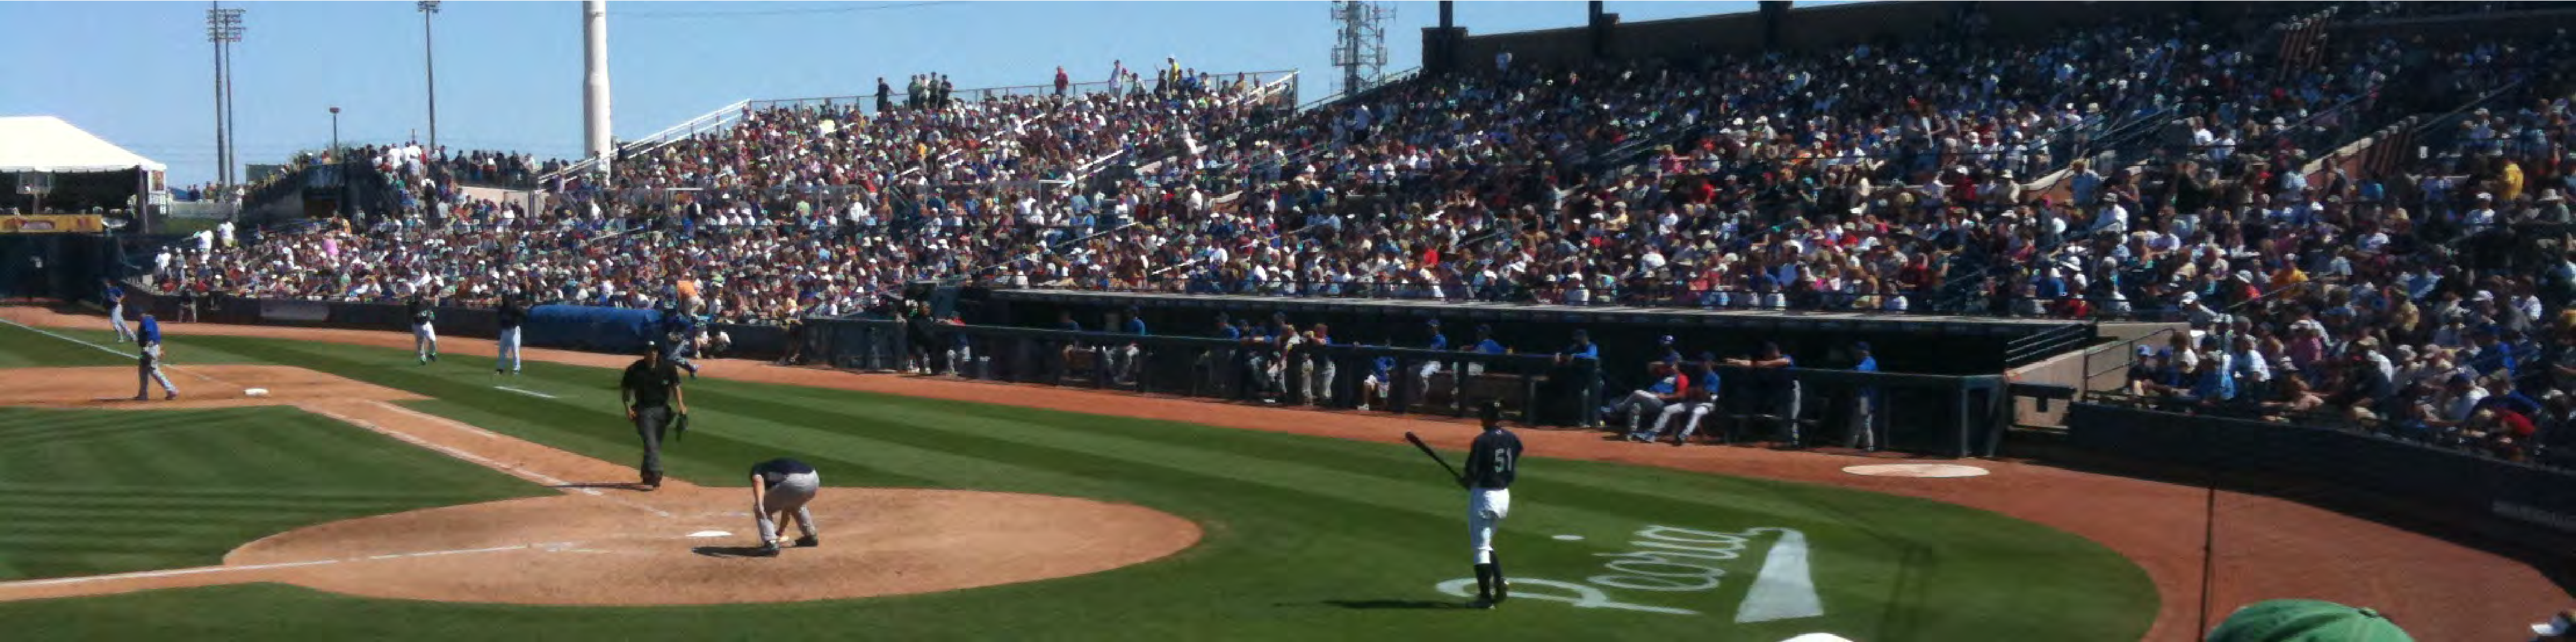
\includegraphics[width=\textwidth]{sampleteaser}
%% \caption{Seattle Mariners at Spring Training, 2010.}
 %% \Description{Enjoying the baseball game from the third-base
 %% seats. Ichiro Suzuki preparing to bat.}
 %% \label{fig:teaser}
%%\end{teaserfigure}

%%
%% This command processes the author and affiliation and title
%% information and builds the first part of the formatted document.
\maketitle

\section{Introduction}

In general, auto-grader's accept user code and perform compilation of the user code, execute the object file generated after compilation and compare the output produced during the execution step with the actual output. The architecture of a typical auto-grader is shown in the figure \ref{typical_auto_grader}, which has a Application Programming Interface, API layer which accepts requests from the users. The service layer executes the auto-grader session i.e compilation, execution and comparing outputs. The database layer is used to store the user related data, produced while running the auto-grader session. After storing the user related data in the database, response is returned to the user through the API layer.
\begin{figure}[h]
  \centering
  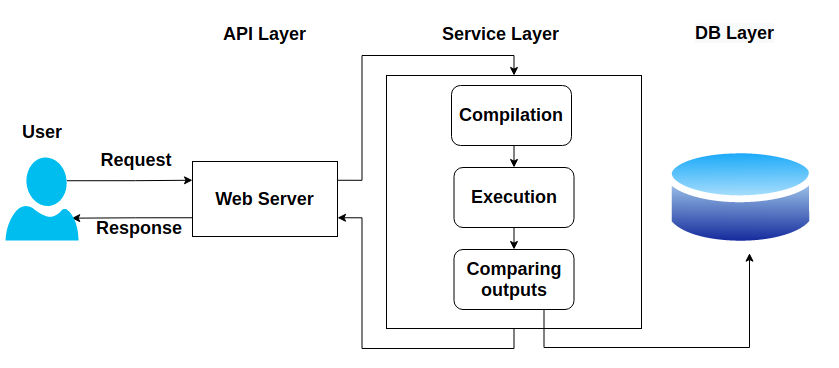
\includegraphics[width=\linewidth]{Pictures/typical_autograder.png}
  \caption{Typical auto-grader architecture}
  \label{typical_auto_grader}
\end{figure}

The challenges with the typical auto-grader architecture shown in the figure \ref{typical_auto_grader}, is that the processing  time of auto-grading session requests depends upon the code the user uploads. Moreover each user code need to run against multiple test cases. Let $n$ be the number of test cases on which the code is run and $Test Case Execution Time(i)$ be the execution time required for the $i^{th}$ test case . As shown in the equation \ref{eq:test_case_execution} the total time required to execute the code is the summation of the time required to execute each test case. Since the resource consumption of different user codes is not the same, the value of $Test Case Execution Time(i)$  will be different among multiple user codes. Therefore the total time required to execute the code will not be the same for different user codes i.e the processing  time of auto-grading session requests is not deterministic.

\begin{equation}
  Total Code Execution Time=\sum_{i=1}^{n} Test Case Execution Time(i)
  \label{eq:test_case_execution}
\end{equation}

If the auto-grading session is processed synchronously then the users have to wait till the response for their request is received, which causes significant number of requests to get timeout when the request load to the auto-grader is high.  Moreover in general the users will resend their requests if they didn't get the response within the time for which they have been patient. Due to non deterministic execution nature of auto-grading session requests, significant number of users may resend their requests which will further increase the request load to the system and worsen the situation. Hence the auto-grading session requests need to be processed asynchronously.


In our Evalpro  application, which is an auto-grader, the auto-grading session i.e compilation, execution and comparing outputs is being processed asynchronously. Even though the request processing is asynchronous, when the load to the system is very high then the system need to gracefully handle the high request load i.e system need to scale its throughput with the request load.  But since the resources of the system are limited, the system will only support up to a certain request load. After a certain request load the throughput of the system  saturates or degrades. The scalability is the the ability of the system to scale its performance proportionally by adding the resources to the system. If there are any software, hardware bottlenecks then the system won't scale its performance proportionally by adding the resources. Therefore identifying the software, hardware bottlenecks which are limiting the scalability of the system and increasing the resources corresponding to the identified bottlenecks will make the system scalable i.e the system will scale its throughput with the request load. 

Since the execution of the auto-grading session is non deterministic, it is impossible to know the resource requirement in prior to handle a certain amount of request load. Hence the scalability of the system is very important to handle the request load gracefully during the peak usage of a application. Initially we have performed baseline experiments on our Evalpro application to find the baseline throughput scalability. Thereafter we performed experiments to identify the software, hardware bottlenecks which limit the scalability of the application. We designed solutions to further avoid the identified bottlenecks and make our Evalpro application to scale its throughput with the request load during its peak usage.

The rest of the paper is organized as follows. In Section \ref{motivation_background} we provide background on our Evalpro architecture, baseline experiment setup and we further motivate our work using the baseline experiment results. A systematic bottleneck analysis to find the reason for limitation in the baseline throughput scalability is briefly described in the Section \ref{baseline_bottleneck_analysis}. Section \ref{horizontal_scalability} describes the usage of Horizontal scalability using Docker swarm, KVM-QEMU virtualization technologies and compares the throughput scalability achieved using them with the baseline throughput scalability. Section \ref{mongodb_filestorage} describes the usage of MongoDB for storing the files into database instead of disk to improve the scalability and compares the throughput scalability achieved using MongoDB with the baseline throughput scalability. In the sections \ref{baseline_64} and \ref{mongo_64_cores},  we perform baseline experiments and the experiments using MongoDB for file storage respectively, on higher number of CPU cores and also compared their throughput scalability. In section \ref{micro_benchmark_exps} we describe about two micro benchmarks i.e CPU micro benchmark and Evalpro micro benchmark which are developed to find the best scalability we can achieve for a raw CPU workload and Evalpro application respectively. A low level bottleneck analysis using PERF tool to find the reason for throughput scalability limitation in the Evalpro application is briefly described in the Section \ref{micro_benchmark_bottleneck_analysis}. Finally we conclude the paper in the section \ref{conclusion}


\section{Background and Motivation} \label{motivation_background}
\subsection{Evalpro Design}
Evalpro is a server based auto-grader application in which auto-grading requests sent by the users are processed at the server. The figure \ref{evalpro_architecture} shows the current architecture of Evalpro application, which runs in the docker [citation] environment, the different components of the application i.e Nginx, HAProxy, Postgress, Redis are isolated by running each component on a separate container. Except that WSGI, Celery components run on same container.

\begin{figure}[h]
  \centering
  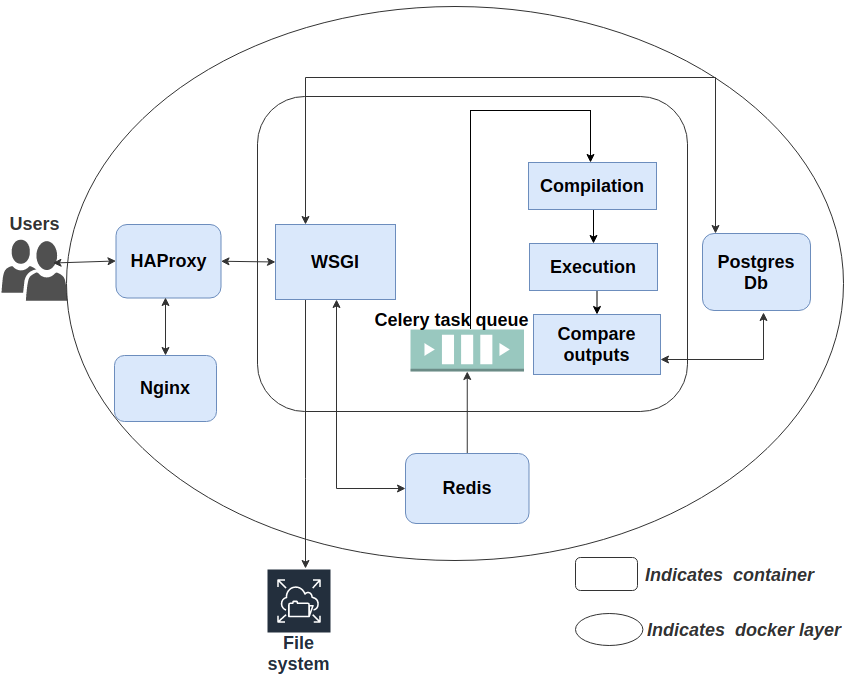
\includegraphics[width=\linewidth]{Pictures/architecture_10.png}
  \caption{Evalpro architecture}
  \label{evalpro_architecture}
\end{figure}

\begin{enumerate}
\item {\texttt{WSGI}}: WSGI stands for Web Server Gateway Interface. It behaves as a internal web server, which accepts HTTP requests sent by
the load balancer. It contains multiple gunicorn workers, where each worker accepts
HTTP requests and process them by sending them into the processing pipeline. 
After completion of request processing, the response is sent back to the users. It also uses file system to store the user uploaded files in the hard disk. 
\item {\texttt{Celery}}: It executes tasks asynchronously by maintaining a task queue, into which the broker en-queue’s the messages i.e task related information. Celery threads will
pick the messages from the queue and asynchronously execute the task’s corresponding to the messages. As shown in the figure \ref{evalpro_architecture} celery threads perform the task of auto-grading session i.e compilation, execution and comparison of outputs asynchronously.  After the task is completed, celery informs the message broker about completion.
\item {\texttt{HAProxy}}: It behaves as a load balancer, which uses the ports exposed by WSGI+Celery replica’s to distribute the requests it received among those replica’s
in a round robin manner. It also plays the role of an external web server which accepts requests from external network and sends the requests for the static content
to static content delivery network(CDN) and the dynamic content to WSGI+Celery
replica’s
\item {\texttt{Redis}}: It acts as a message broker, which en-queue’s the tasks into the celery task queue. If the task queue is configured to be persistent then while en-queuing a task into the task queue, it also maintains the task information in a file. This will be helpful when some tasks fail to complete due to system crashes, broker will again en-queue the requests related to those tasks to the task queue.
\item {\texttt{Postgres}}: It is a database server which processes queries related to fetching data from the database and storing data to the database. It maintains application data in a structured manner using tables. The tables are related to each other by foreign keys.
\item {\texttt{Nginx}}: It acts as a static Content Delivery Network (CDN), which process the requests related to the static data, for example fetching HTML, JavaScript files.

\end{enumerate}

Using this  architecture we have performed baseline experiments to find the current scalability of our Evalpro application. The section \ref{baseline_experiemnt_setup} i.e the next section discuss about our experiment setup to perform baseline experiments. The section \ref{baseline_16} further motivates our work by discussing about the baseline experiment results.

\subsection{Baseline Experiment setup}\label{baseline_experiemnt_setup}
We have designed a realistic user session using JMeter to perform experiments on our Evalpro application.
\begin{figure}[!htb]
  \centering
  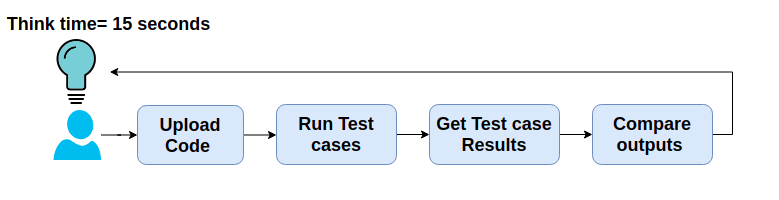
\includegraphics[width=\linewidth]{Pictures/user_session.png}
  \caption{JMeter user session}
  \label{user_session}
  \Description{Realistic user session using JMeter}
\end{figure}
As shown in the figure \ref{user_session}, the user session is simulated with JMeter consists of following steps
\begin{itemize}
\item {\texttt{Upload Code}}: Upload the code in a file by clicking upload button from the user Interface.
 \item {\texttt{Run Test cases}}: Run the user code uploaded in the above step on the available test cases.
\item {\texttt{Get Test case Results}}: After the test cases execution gets completed in the above step. A page will be displayed to the user which shows results of the test cases execution
\item {\texttt{Compare outputs}}: Using the page displayed in the above step, for each test case the output of the uploaded code is compared with the actual output.
\item {\texttt{Think time}}: It is the time for which the user waits before starting  user session for the next time. We have configured the think time to be 15 seconds for our experiments.
\end{itemize}
\begin{figure}[!htb]
  \centering
  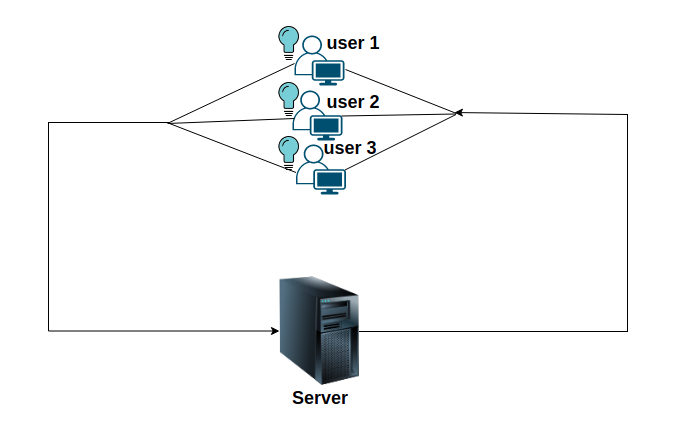
\includegraphics[width=\linewidth]{Pictures/closed_loop.png}
  \caption{Closed load system}
  \label{closed_system}
  \Description{Realistic user session using JMeter}
\end{figure}

\begin{table*}
  \begin{tabular}{ccccc}
    \toprule
    Type&CPU&Cores&Memory&CPU Cache\\
    \midrule
    Server & Intel(R) Xeon(R) CPU E5-2650 v2 @ 2.60GHz& 16&16GB&20MB\\
    Client & AMD Opteron(TM) Processor 6212 & 16&16GB&8MB\\
  \bottomrule
\end{tabular}
\caption{Hardware specifications}
  \label{tab:hardware}
\end{table*}

As shown in the figure  \ref{closed_system}, a closed load system is created in which  the above described user session is run simultaneously by creating multiple users using JMeter  on the client machine and the Evalpro application is run on the sever machine which accepts requests sent by multiple users from the client machine. The generation of the load from the client is configured to run for 5 minutes using JMeter. During the load test, server performance metrics are collected using various Linux utilities i.e vmstat for CPU utilization,iostat for disk utilization, netstat for network bandwidth and the request throughput and latency are collected by JMeter. The table \ref{tab:hardware} shows various hardware specifications of the client and the server machines.

Using this experiment setup, we have performed the baseline experiments to find the current scalability of the Evalpro application. The next section briefly describes about the baseline experiment results.

\subsection{Baseline Experiments}\label{baseline_16}
Using the above experiment setup shown in the figure \ref{closed_system}, in our baseline experiments to avoid the apparent bottlenecks,  we have configured number of celery  threads equal to the number of CPU cores, number of postgres connections to 10000, a relatively higher number compared to the default value of 100. We have performed experiments by altering the number of CPU cores available.

The observed throughput is the throughput we observed from our experiments. The ideal throughput with $N$ CPU cores is the desired throughput, which is equal to $N*Throughput_{max}(1)$. The observed value of $Throughput_{max}(1)$ is 0.3 requests per second. As shown in the figure \ref{baseline_throughput_plot}, when the number of CPU cores $N$ increases, the maximum throughput observed with $N$ CPU cores, $Throughput_{max}(N)$ increases linearly up to $N=8$ CPU cores. When the number of CPU cores $N>8$, then the difference between the values of the observed  $Throughput_{max}(N)$  and the ideal $Throughput_{max}(N)$ is significantly high i.e the throughput is not scaling linearly.


\begin{figure}[!htb]
  \centering
  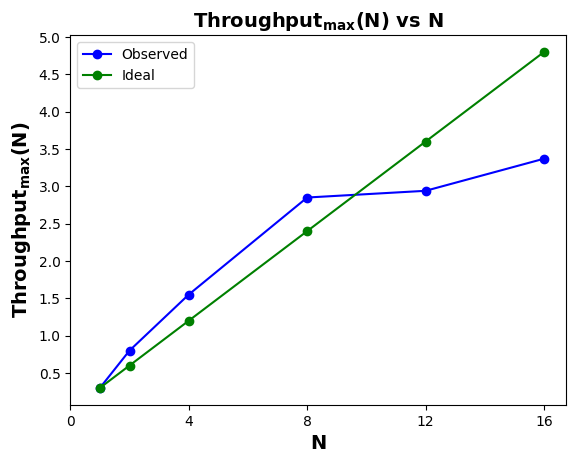
\includegraphics[width=\linewidth]{Pictures/baseline_16_cores.png}
  \caption{Baseline Throughput plot}
  \label{baseline_throughput_plot}
  \Description{Baseline Throughput plot}
\end{figure}


To measure how well the scaling of the throughput is happening we used scalability factor. As shown in the equation \ref{eq:1}, the scalability factor for $N$ CPU cores is  $S(N)$, which is equal to the ratio of the maximum throughput observed with $N$ CPU cores,  $Throughput_{max}(N)$ and the maximum throughput observed with a single CPU core $Throughput_{max}(1)$.
\begin{equation}
  S(N)=\frac{Throughput_{max}(N)}{Throughput_{max}(1)}
  \label{eq:1}
\end{equation}

For our baseline experiments we have calculated $S(N)$ value for different values of $N$, the number of CPU cores. The scalability factor we got for 16 CPU cores is 11.2, but the ideal value of S(16) is 16. It is clear that the throughput scalability of the Evalpro application is not scaling proportionally with increase in the number of CPU cores. To get the linear scaling of the throughput  $S(N)$ should be as close as $N$. 

In general, the scalability limitation of an application is due to some underlying bottlenecks in the closed load system which make the application's performance not to  scale proportionally with increase in the hardware resources. Therefore we hypothesise that there are some bottlenecks  which are limiting the scalability of the Evalpro application. Some examples of bottlenecks include insufficient threads for processing, lock contention of software, hardware resources. To find the bottlenecks and improve the current baseline scalability, we have done bottleneck analysis on the baseline experiment setup by tuning different software components of the Evalpro application. The next section briefly describes about the baseline bottleneck analysis on the Evalpro application.

\section{Baseline Bottleneck Analysis}\label{baseline_bottleneck_analysis}
As shown in the previous section the throughput of Evalpro application didn't scale proportionally with increase in the number of CPU cores. Based on our hypothesis at the end of our previous section, in this section we have done bottleneck analysis on the Evalpro application to find the reason for limitation in the current scalability and improve it. To find the bottlenecks and improve the current baseline scalability, we have performed the following experiments  by tuning performance parameters of different software components.
\begin{itemize}
    \item
    Increasing gunicorn workers
    \item
    Modifying celery threads
    \item
    Setting CPU affinities to celery threads
    \item
    Disabling writing to log files
    \item
    Modifying Celery Prefetch multiplier
    \item
    Increasing celery broker pool limit
    \item
    Using transient celery queue
\end{itemize}

\subsection{Increasing gunicorn workers:}
Gunicorn workers are part of WSGI, which accepts HTTP requests sent by the users and send them into the execution pipeline. The number of gunicorn workers for the baseline experiments is 10. We tried to modify the number of gunicorn workers to see improvement in $S(N)$ for $N>8$. When the number of CPU cores $N$ is equal to 16 we have modified the number gunicorn workers configuration. As shown in the figure \ref{gunicorn_plot} when the number of gunicorn workers increased the value of $S(16)$, almost remains constant. By this we can say that tuning the number of gunicorn workers doesn't improve  $S(N)$ for $N>8$.
\begin{figure}[!htb]
  \centering
  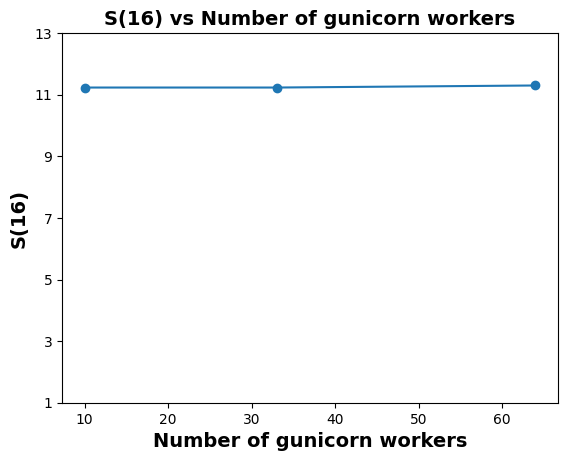
\includegraphics[width=\linewidth]{Pictures/gunicorn_workers.png}
  \caption{Tuning Gunicorn workers}
  \label{gunicorn_plot}
  \Description{Gunicorn workers tuning plot}
\end{figure}
\subsection{Modifying celery threads:}
Celery threads pick the tasks which are en-queued into the celery queue by the message broker, Redis and executes those tasks asynchronously. In our Evalpro application the task of auto-grading session is performed asynchronously by the celery threads. The number of celery threads for the baseline experiments is equal to $N$, the number of CPU cores. We tried to modify the number of celery threads to see improvement in $S(N)$ for $N>8$. When the number of CPU cores $N$ is equal to 16,  we have modified the number of celery threads. As shown in the figure \ref{celery_plot}, when the number of celery threads are less than 16, S(16) value is less than the baseline value 11.2. Moreover from the CPU utilization plot in the figure \ref{celery_plot} it is clear that when the number of celery threads are less than $N$, they are becoming the bottleneck making the CPU not to utilize completely. When the celery threads count is greater than 16, S(16) value almost remained constant. By this we can say that increasing the celery threads count beyond $N$ doesn't improve $S(N)$.
\begin{figure}[!htb]
  \centering
  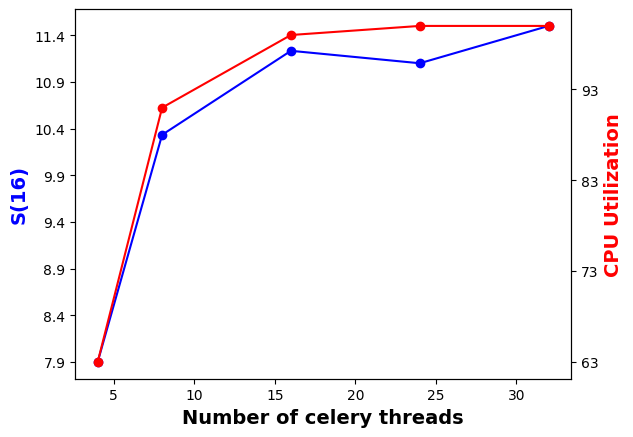
\includegraphics[width=\linewidth]{Pictures/celery_threads.png}
  \caption{Tuning Celery threads}
  \label{celery_plot}
  \Description{Tuning Celery threads}
\end{figure}
\subsection{Setting CPU affinities to celery threads:}
When each thread is run on a different CPU core, there will be less inter core contention. Due to which we hypothesised that setting CPU affinities to celery threads will improve  $S(N)$ for $N>8$. When the number of CPU cores $N$ is equal to 16, we have pinned each celery threads to a CPU core but observed no improvement in $S(16)$.
\subsection{Disabling writing to log files:}
During the processing of requests by the Evalpro application, useful metadata regarding request processing is logged into files by the application at different stages of processing. We hypothesised that due to logging CPU is doing work which is not useful. so, to see improvement in $S(N)$ for $N>8$, we disabled writing to gunicorn access log and celery log files. After disabling logging, we performed experiment when the number of CPU cores $N$ is equal to 16 and measured $S(16)$ value, which came out to be 11, very close to baseline value 11.2. By this we can say that disabling writing to log files  doesn't improve $S(N)$ for $N>8$.
\subsection{Modifying celery prefetch multiplier:}
Prefetch multiplier is the number of tasks each celery thread fetches at a time from the queue and keeps in the memory instead of going to queue and fetching the task every time. For our baseline experiments the prefetch multiplier value is 4.  We have modified the value of prefetch multiplier  to see improvement in $S(N)$ for $N>8$. When the number of CPU cores $N$ is equal to 16,  we have modified the value of prefetch multiplier.  As shown in the figure \ref{prefetch_multiplier_plot} when the value of  prefetch multiplier changed, the value of $S(16)$,  almost remains constant. By this we can say that tuning the value of prefetch multiplier doesn't improve  $S(N)$ for $N>8$.
\begin{figure}[!htb]
  \centering
  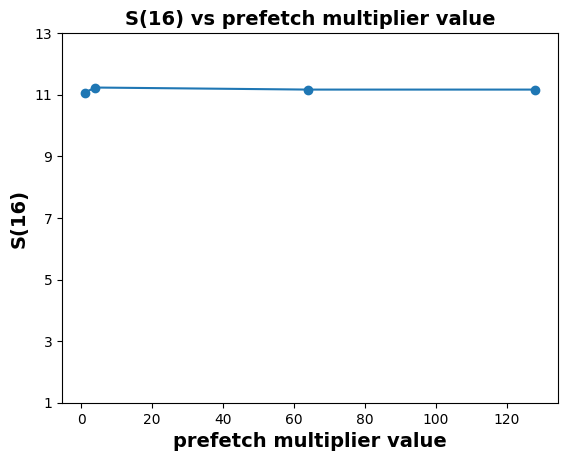
\includegraphics[width=\linewidth]{Pictures/prefetch_multiplier.png}
  \caption{Tuning Celery Prefetch multiplier}
  \label{prefetch_multiplier_plot}
  \Description{Tuning Celery Prefetch multiplier}
\end{figure}
\subsection{Increasing celery broker pool limit}
Broker pool limit is the number of connections celery keeps open instead of creating new connection for every task en-queued into the celery task queue by the message broker,Redis. The celery broker pool limit for the baseline experiments is 10. We tried to modify this value to see improvement in $S(N)$ for $N>8$. When the number of CPU cores $N$ is equal to 16 we have modified the broker pool limit configuration. As shown in the figure \ref{broker_pool_limit} when the broker pool limit is increased the value of $S(16)$, almost remains same as baseline $S(16)$ value. By this we can say that tuning the broker pool limit doesn't improve  $S(N)$ for $N>8$.
\begin{figure}[!htb]
  \centering
  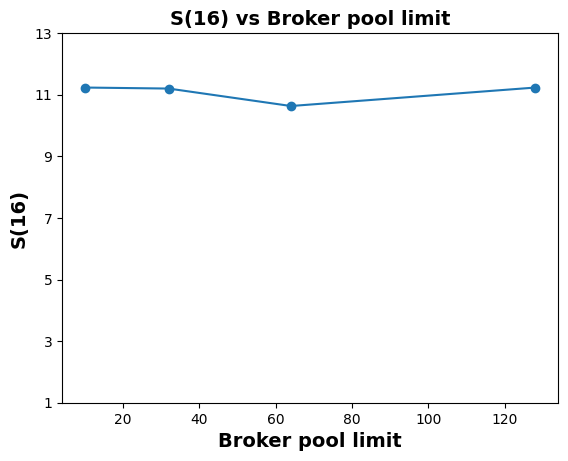
\includegraphics[width=\linewidth]{Pictures/broker_limit.png}
  \caption{Tuning Broker pool limit}
  \label{broker_pool_limit}
  \Description{Tuning Celery threads}
\end{figure}
\subsection{Using transient celery queue}
By default celery queue is persistent, the task information is logged
into a file by the message broker,Redis when the task is en-queued into the celery task queue. Persistent queues are useful when the system crashes occur, the broker will  use the file to en-queue the failed tasks into the celery 
task queue. To see the improvement in $S(N)$ for $N>8$, we have made the celery task queue transient when the number of CPU cores $N$ is equal to 16 but observed no improvement in $S(16)$. By this we can say that using transient celery queue doesn't improve  $S(N)$ for $N>8$.


From the results of the above experiments it is clear that tuning performance parameters of different software components didn't improve the current baseline scalability. We also have observed that when the throughput achieved is maximum, the CPU utilization of the server is around 90-100\% . Therefore we came to the conclusion  that there are no application bottlenecks, from which we came to the hypothesis that, the isolation between the software,hardware resources improves scalability. So, we have tried horizontal scalability to achieve better scalability factor, $S(N)$ for $N>8$.  The next section briefly describes about the usage of horizontal scalability for our Evalpro application.

\section{Horizontal Scalability} \label{horizontal_scalability}
Horizontal scalability is the ability of the system to scale its performance  when a new application replica is added which consists a new set of hardware resources i.e CPU, memory or disk. The load balancer will distribute the load across multiple replicas. We have used two different virtualization techniques, Containers and Virtual machines for Horizontal scalability.
\subsection{Horizontal scaling with Containers}
Docker has inbuilt cluster management and orchestration framework, docker swarm. As shown in the figure \ref{docker_swarm}, using docker swarm multiple replicas of WSGI+Celery container replicas are created with each replica assigned with different CPU cores. Moreover each container replica will have a different PID namespace. Thus the isolation with containers is more compared to the baseline experiments. The HAProxy will balance the request load from the users  in a round robin manner across different WSGI+Celery replicas.

As shown in the figure \ref{docker_swarm}, when the number of CPU cores $N$ is equal to 16, 4 WSGI+Celery replicas are created with each replica assigned with 4  different CPU cores. Using this experiment setup, we performed experiments and found that the scalability factor with 16 CPU cores, $S(16)$ value is 11.33 which is almost same as the baseline $S(16)$ value. By this we can say that scaling the Evalpro application horizontally using containers doesn't improve  $S(N)$ for $N>8$.
\begin{figure}[!htb]
  \centering
  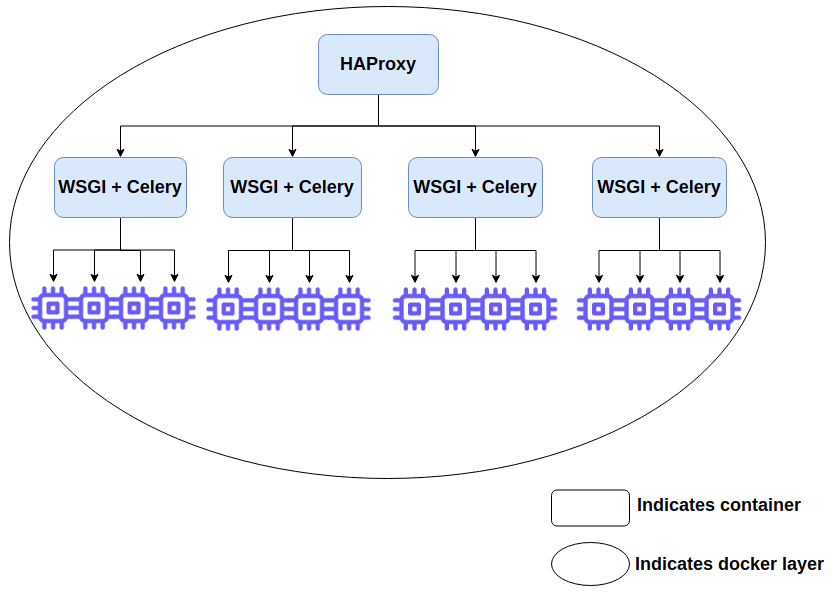
\includegraphics[width=\linewidth]{Pictures/docker_swarm.png}
  \caption{Horizontal scaling with docker}
  \label{docker_swarm}
  \Description{Docker swarm working}
\end{figure}

\subsection{Horizontal scaling with Virtual Machines}
We have used KVM-QEMU, which is a hardware assisted virtualization technique for scaling horizontally using Virtual machines. Using KVM-QEMU hypervisor multiple VM's can be created with each VM assigned with different set of CPU cores. Moreover each VM can get its own share of the RAM and the Disk. Thus the isolation with VM's is more than containers and the baseline experiments. The isolation of the hardware resources between VM's is managed by the KVM-QEMU hypervisor.
\subsubsection{Completely Isolated setup:}
As shown in the figure \ref{isolated_vm}, when the number of CPU cores $N$ is equal to 16, 2 VM's are created with each replica assigned with 8  different CPU cores, 8GB RAM and 30GB hard disk. Evalpro instance is run on each VM in an completely isolated manner. Using this experiment setup, we have performed experiments and found that the $S(16)$ value is 14.8 which is significantly more than the baseline $S(16)$ value,11.2. All the CPU cores in both VM's have been completely utilized. But in this setup each Evalpro instance has separate  Postgres database which constitutes to the following limitations
\begin{figure}[!htb]
  \centering
  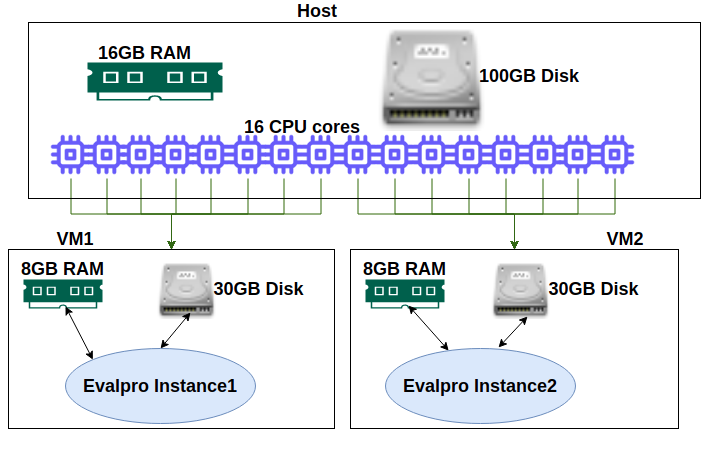
\includegraphics[width=\linewidth]{Pictures/isolated_vm.png}
  \caption{Isolated VM setup}
  \label{isolated_vm}
  \Description{Isolated VM setup}
\end{figure}
\begin{itemize}
    \item 
    Separate user related data should be maintained for each Evalpro instance
    and the load balancer need to maintain information about to which instance it has to forward the request, so that the user gets the correct response.
    \item
    Moreover when the request load is high i.e the VM's are completely utilized, adding a new VM to scale the performance of the system, requires migration of the part of user data to the new VM from the old VM's, which is a very complex as the tables in Postgres database are related to each other by the foreign keys.
\end{itemize}

Due to the above limitations, it is very complex and infeasible to use Isolated VM setup. So, we have shared the user related data,files among multiple VM's so that the load balancer need not maintain request to instance mapping, it can distribute the user requests to multiple VM's in a round robin manner and new VM's can be added to scale the performance of the system without any requirement of the migration of the user data. The next section briefly describes about this experiment setup.
\subsubsection{User Data and Files sharing setup:}
As shown in the figure \ref{shared_vm}, Postgres Database  and the Media folder which consists of the files uploaded by the user for running code is shared among the two VM's. Media folder is placed in the Host machine and mounted on both the VM's so that the both the VM's can share the Media folder to store user uploaded files. Using this experiment setup, we have performed experiments and found that the  $S(16)$ value is 9.2 which is significantly less than the baseline $S(16)$ value,11.2. Moreover all the CPU cores in both VM's have not been completely utilized i.e 80\% utilized.
\par
Thus with the above experiment results, we came to conclusion that with the shared VM setup there are some bottlenecks which are making the Evalpro application not to scale. The next section briefly describes about our approach to find the bottlenecks with this experiment setup.
\begin{figure}[!htb]
  \centering
  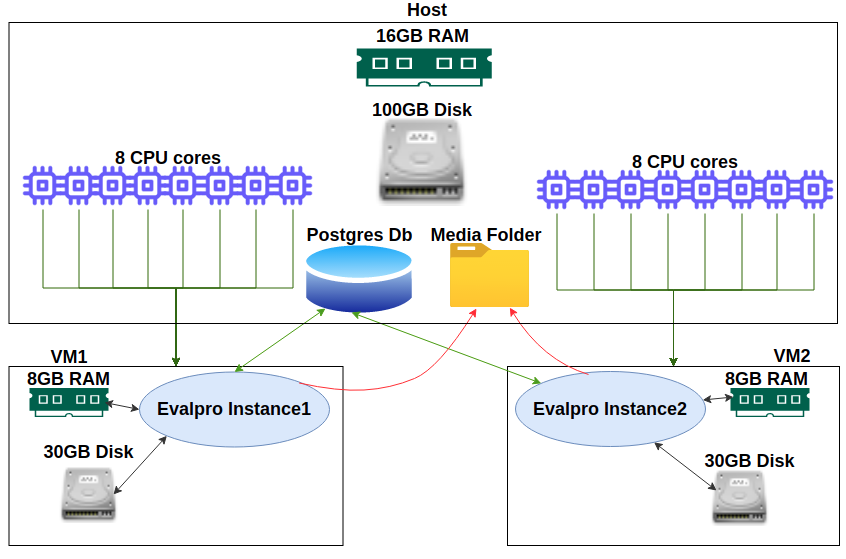
\includegraphics[width=\linewidth]{Pictures/shared_vm.png}
  \caption{Shared VM setup}
  \label{shared_vm}
  \Description{Shared VM setup}
\end{figure}
\subsection{Shared VM Bottleneck Analysis}
To find the bottlenecks which are limiting the scalability of the Evalpro application observed in the above section, we have divided the current user session shown in the figure \ref{user_session}, into the following parts.
\begin{enumerate}
    \item {\texttt{Without Upload:}} As shown in the figure \ref{without_upload_session}, this user session consists of all the steps in the current user session shown in the figure  \ref{user_session}, except the step in which the user uploads the code. Since there is no file upload,  we have reduced the think time of the user to 8 seconds from 15 seconds.
    \begin{figure}[!htb]
  \centering
  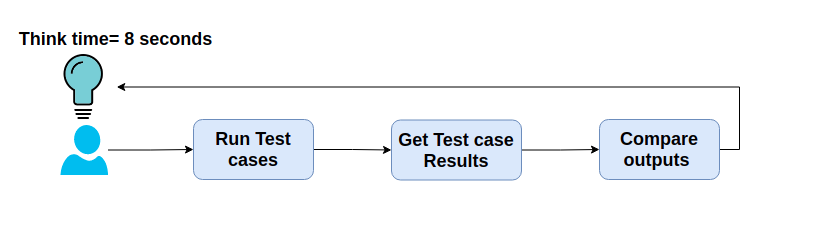
\includegraphics[width=\linewidth]{Pictures/with_out_upload_session.png}
  \caption{User session without upload}
  \label{without_upload_session}
  \Description{User session without upload}
\end{figure}
    \item {\texttt{Only Upload:}} As shown in the figure \ref{upload_session}, this user session only consists of the step where the user uploads the code. We have configured the user think time to be same as the  current user session, shown in the figure \ref{user_session} i.e 15 seconds.
    \begin{figure}[!htb]
  \centering
  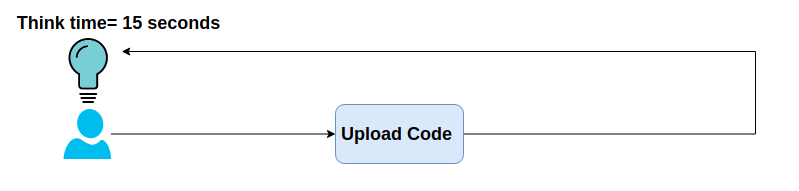
\includegraphics[width=\linewidth]{Pictures/only_upload_session.png}
  \caption{User session with only upload}
  \label{upload_session}
  \Description{User session with only upload}
\end{figure}
\end{enumerate}




Using the \texttt{Without Upload}  user session shown in the figure \ref{without_upload_session}, we have performed experiments on a single CPU core. The maximum throughput achieved on a single CPU core, $Throughput_{max}(1)$ was observed to be 1.35 requests per second. With the shared VM experiment setup shown in the figure \ref{shared_vm}, we performed experiments and found that the maximum throughput achieved on the 16 CPU cores, $Throughput_{max}(16)$ to be 17.31 requests per second. We calculated $S(16)$, the scalability factor with 16 CPU cores using the equation \ref{eq:1}, by which  the $S(16)$ value is 13, which is close to the ideal $S(16)$ value 16.

Same experiments described above are performed using \texttt{Only Upload} user session shown in the figure \ref{upload_session} , in which the single CPU core maximum throughput,  $Throughput_{max}(1)$ was observed to be 1.26 requests per second.  With the shared VM experiment setup shown in the figure  \ref{shared_vm}, the  maximum throughput with 16 CPU cores, $Throughput_{max}(16)$  was observed to be 5.91 requests per second. Therefore by using the equation \ref{eq:1}, the Scalability factor with 16 CPU cores, $S(16)$ value is 4.71.


\begin{figure}[!htb]
  \centering
  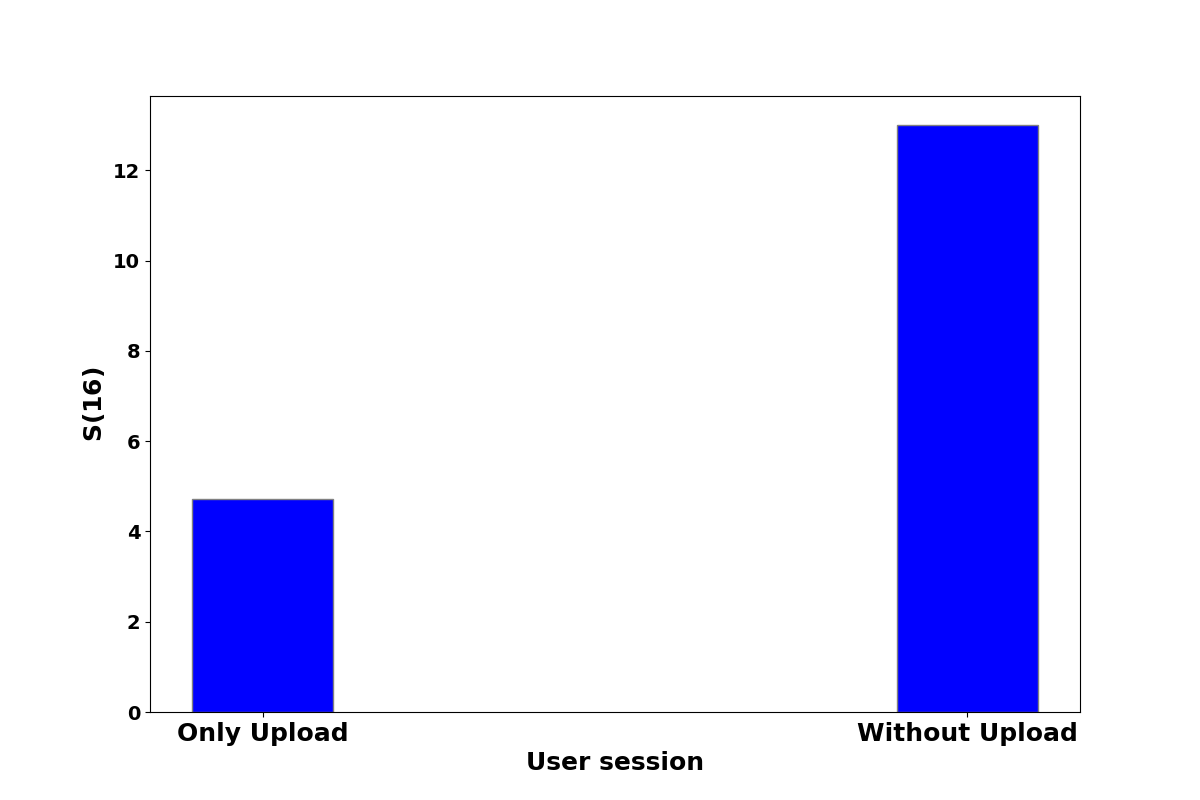
\includegraphics[width=\linewidth]{Pictures/upload_vs_without_upload.png}
  \caption{Scalability for different User sessions}
  \label{compare_user_sessions}
  \Description{Comparing the scalability for different User sessions}
\end{figure}

By comparing the $S(16)$  value calculated above for \texttt{Without Upload} and  \texttt{Only Upload} user sessions shown in the figure  \ref{compare_user_sessions} , we observed that for \texttt{Only Upload} user session the scalability  of the Evalpro application is very less compared to \texttt{Without Upload}. Moreover the CPU utilization of the server for  \texttt{Only Upload} user session  didn't exceed beyond 35\%, which also confirms that uploading file is the bottleneck. From these results we came to the conclusion that for the combined user session shown in the figure \ref{user_session}, using shared VM setup shown in the figure \ref{shared_vm}, file upload is becoming the bottleneck because uploading a file in the Media folder which is in the host requires each VM to make a world switch[citation] to the Host and upload file in the Media folder, which is a significant overhead

Therefore we hypothesise that with the shared VM setup shown in the figure \ref{shared_vm},  using database to store the uploaded files instead of disk will improve the scalability factor $S(N)$ for $N>8$, because there is no need for VM's to make a world switch to the host to upload a file,  when the files are stored in the  database, shared between VM's. So, we used MongoDB database to store the uploaded files. The next section briefly describes about the experiments performed on the Evalpro application using MongoDB to store the files uploaded by the user.

\section{MongoDB for File Storage}\label{mongodb_filestorage}
MongoDB is a NO-SQL database. It stores data in unstructured manner using key,value pairs. Based on our hypothesis from the above experiments we used MongoDB to store the user uploaded files. As shown in the figure \ref{architecture_mongo}, we have modified the current Evalpro architecture shown in the figure \ref{evalpro_architecture} by replacing the file system with MongoDB to store the files uploaded by the user. We have performed our experiments on this new Evalpro architecture to see the improvement in $S(N)$ for $N>8$. We also have changed the experiment setup with VM's, as shown in the figure \ref{shared_vm_mongo}, MongoDB is shared between VM's in place of the Media folder. 

\begin{figure}[!htb]
  \centering
  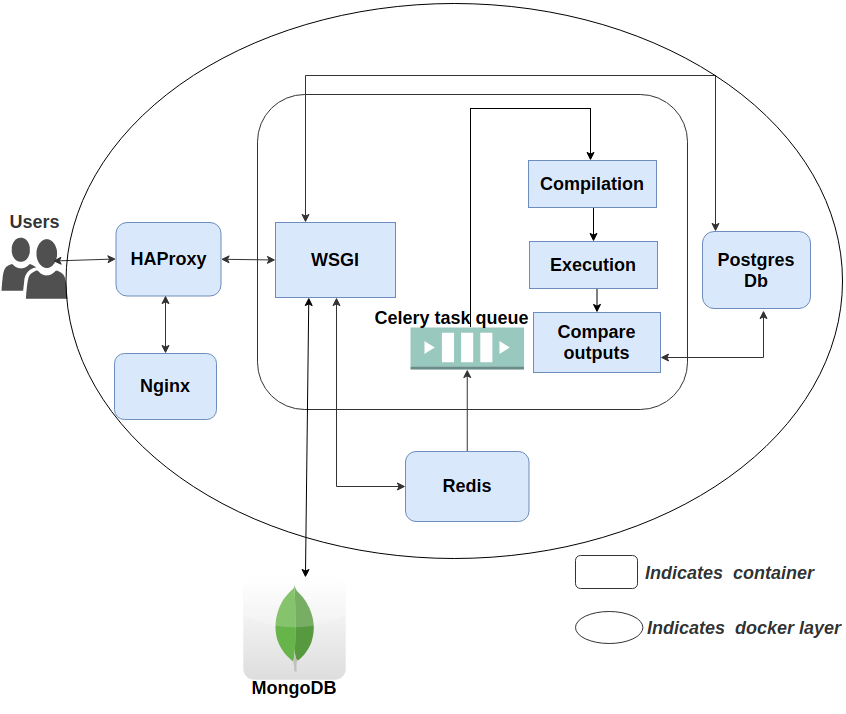
\includegraphics[width=\linewidth]{Pictures/architecture_mongo.png}
  \caption{Evalpro new architecture}
  \label{architecture_mongo}
  \Description{Evalpro new architecture using MongoDB}
\end{figure}

\begin{figure}[!htb]
  \centering
  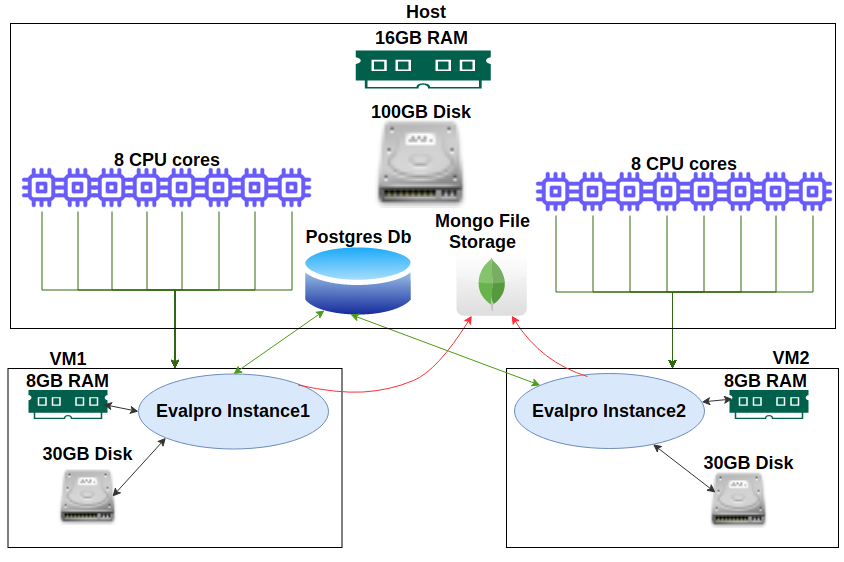
\includegraphics[width=\linewidth]{Pictures/shared_vm_mongo.png}
  \caption{Shared VM setup with  MongoDB}
  \label{shared_vm_mongo}
  \Description{Shared VM setup with  MongoDB}
\end{figure}

Using the combined user session shown in the figure \ref{user_session}, we have performed experiments with the new Evalpro architecture on a single CPU core. The maximum throughput achieved on the single CPU core, $Throughput_{max}(1)$ was observed to be 0.29 requests per second. Using the MongoDB with the shared VM experiment setup shown in the figure \ref{shared_vm_mongo}, we performed experiments and found that the maximum throughput achieved on the 16 CPU cores, $Throughput_{max}(16)$ to be 3.51 requests per second, which is slightly higher than the baseline $Throughput_{max}(16)$ 3.37 requests per second . We calculated $S(16)$, the scalability factor with 16 CPU cores using the equation \ref{eq:1}, by which the $S(16)$ value is 12  slightly higher than the baseline $S(16)$ value 11.2.

Even though the improvement in  $Throughput_{max}(16)$ and $S(16)$  we observed is very low using MongoDB, with the shared VM setup shown in the figure \ref{shared_vm_mongo}. we hypothesise that when the number of CPU cores, $N$ is high i.e 64 cores, then  using the MongoDB, with the shared VM experiment setup will significantly improve the throughput, $Throughput_{max}(N)$ and  the scalability factor, $S(N)$ compared to the baseline values of the throughput and the scalability factor respectively . To validate this hypothesis, we performed experiments using a sever machine having 64 CPU cores. The coming sections briefly describes about these experiments.

\section{Baseline Experiments on 64 cores}\label{baseline_64}
As shown in the table \ref{tab:hardware_64_cores}, the server on which Evalpro application is running now has 64 CPU cores. Using which we have performed the baseline experiments on the Evalpro architecture shown in the figure \ref{evalpro_architecture}, with the user session shown in the figure \ref{user_session}. We have performed experiments by altering the number of CPU cores available. The observed throughput is the throughput we observed from our experiments. The ideal throughput with $N$ CPU cores is the desired throughput which is equal to $N*Throughput_{max}(1)$. The observed value of $Throughput_{max}(1)$ is 0.66 requests per second.

\begin{table*}[!htb]
  \begin{tabular}{ccccc}
    \toprule
    Type&CPU&Cores&Memory&CPU Cache\\
    \midrule
    Server & Intel(R) Xeon(R) CPU E5-2683 v4 @ 2.10GHz& 64&128GB&88MB\\
    Client & AMD Opteron(TM) Processor 6212 & 16&16GB&8MB\\
  \bottomrule
\end{tabular}
\caption{Hardware specifications}
  \label{tab:hardware_64_cores}
\end{table*}

As shown in the figure \ref{baseline_throughput_64_cores}, when the number of CPU cores $N$ increases, the maximum throughput achieved with $N$ CPU cores, $Throughput_{max}(N)$ increases. But when the number of CPU cores $N>32$,  then the difference between the values of the observed  $Throughput_{max}(N)$  and the ideal $Throughput_{max}(N)$ is significantly high i.e throughput is not scaling linearly.

To measure the scaling of throughput, we calculated the scalability factor with $N$ CPU cores, $S(N)$ using the equation \ref{eq:1}. The scalability factor we got for 64 CPU cores is 30, but the ideal  S(64) value is 64. By these results we can say that the system is not scaling proportionally with the baseline setup. Moreover when the throughput achieved is maximum, the CPU utilization of the server is around 90-100\%. By this we came to conclusion that there are no application bottlenecks. 

\begin{figure}[!htb]
  \centering
  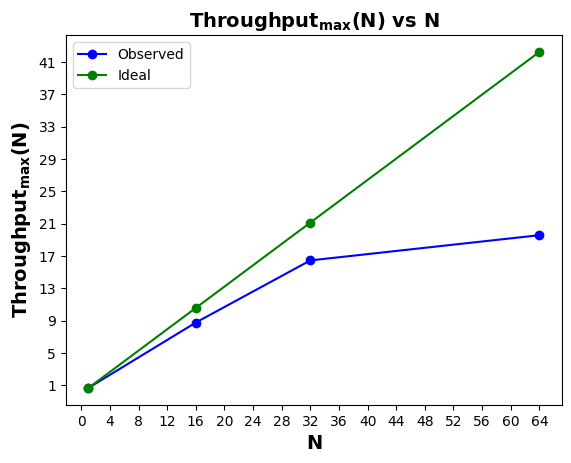
\includegraphics[width=\linewidth]{Pictures/baseline_64_cores.png}
  \caption{Baseline throughput plot with 64 cores}
  \label{baseline_throughput_64_cores}
  \Description{Baseline throughput plot with 64 cores}
\end{figure}

Based on our hypothesis at the end of previous section, to see the improvement in both  $S(N)$ and $Throughput_{max}(N)$, when the number of CPU cores $N>32$, we performed experiments using MongoDB, with the shared VM setup shown in the figure \ref{shared_vm_mongo} on 64 CPU cores. The next section briefly describes about these experiments.

\section{MONGODB FOR FILE STORAGE on 64 Cores}\label{mongo_64_cores}
The experiments in the section \ref{mongodb_filestorage} are performed on the new server machine having 64 CPU cores, which is shown in the table \ref{tab:hardware_64_cores}. As shown in the figure \ref{shared_vm_mongo_64_cores}  4 VM's are created with each VM assigned with 16  different CPU cores, 32GB RAM and 100GB hard disk and the Evalpro application instance is run on each VM.



\begin{figure}[!htb]
  \centering
  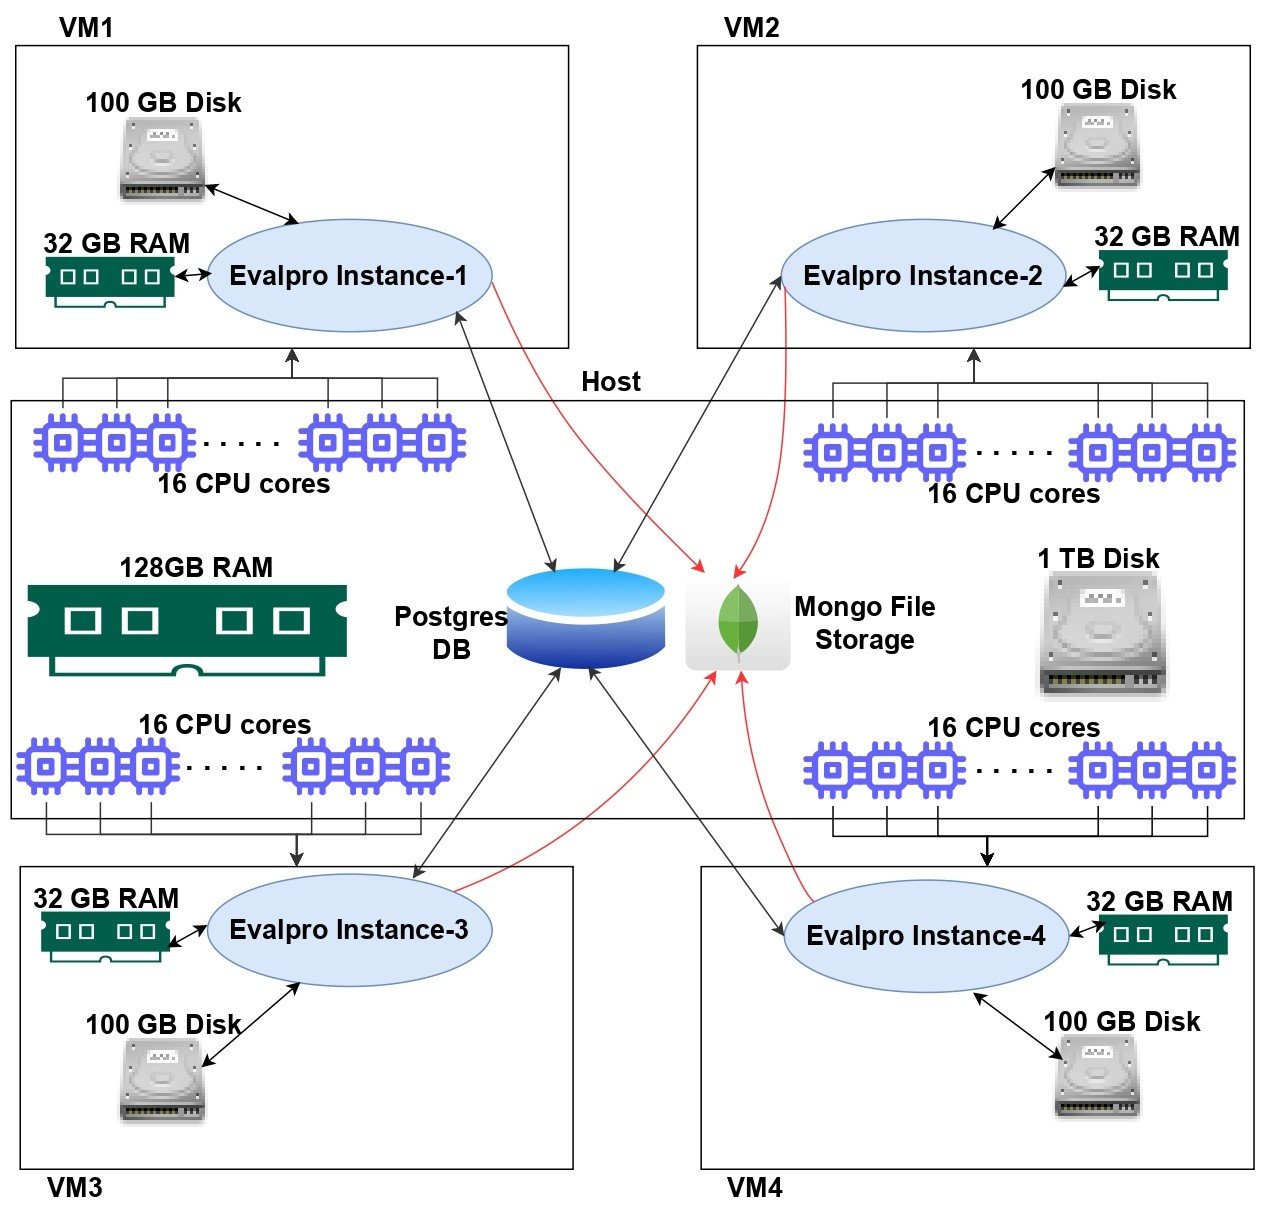
\includegraphics[width=\linewidth]{Pictures/shared_vm_mongo_64_cores.png}
  \caption{Shared VM setup with MongoDB(64 cores)}
  \label{shared_vm_mongo_64_cores}
  \Description{Shared VM setup with MongoDB (64 cores)}
\end{figure}

Using the user session shown in the figure \ref{user_session}, we have performed experiments with the new Evalpro architecture which uses MongoDB for file storage, shown in the figure \ref{architecture_mongo}, on a single CPU core. The maximum throughput achieved on the single CPU core, $Throughput_{max}(1)$ was observed to be 0.47 requests per second. Using MongoDB with the shared VM experiment setup shown in the figure \ref{shared_vm_mongo_64_cores}, we performed experiments and found that the maximum throughput achieved on the 64 CPU cores, $Throughput_{max}(64)$ to be 11.27 requests per second, which is less than the baseline $Throughput_{max}(64)$ 19.56 requests per second . We calculated $S(64)$, the scalability factor with 64 CPU cores using the equation \ref{eq:1}, by which the $S(64)$ value is 24, which is less than the baseline $S(64)$ value 30.

By the above results, we came to conclusion that our hypothesis, when the number of CPU cores, $N$ is high i.e 64 cores, the value of  $Throughput_{max}(N)$ and $S(N)$ using MongoDB, with the shared VM experiment setup will be significantly higher than the baseline  $Throughput_{max}(N)$ and $S(N)$ values respectively, is wrong.

To find the best scalability  of the Evalpro application on a given platform, we have developed micro benchmarks, which depicts whether the limitation in the scalability is due to the Evalpro application or inherent to the platform. The next section briefly describes about the micro-benchmark experiments.

\section{Micro benchmark Experiments}\label{micro_benchmark_exps}
Micro benchmarks are simple, lightweight, portable benchmarks for establishing the best
scalability of the workload for a given platform, which are used to isolate whether scalability limit is due to the application, or inherent to the platform. We have developed two different types of micro benchmarks i.e CPU micro benchmark and Evalpro micro benchmark. The coming sections briefly describes about them.
\subsection{CPU micro benchmark}
To find the best scalability we can get for a raw CPU workload, a completely CPU bound benchmark is created with consists a tight loop of 200 iterations, each iteration runs the CPU bound job, which increments a counter in the loop for large number  of iterations i.e 100000000. The CPU micro benchmark is run on the server having 64 CPU cores shown in the table \ref{tab:hardware_64_cores}. 

\begin{figure}[!htb]
  \centering
  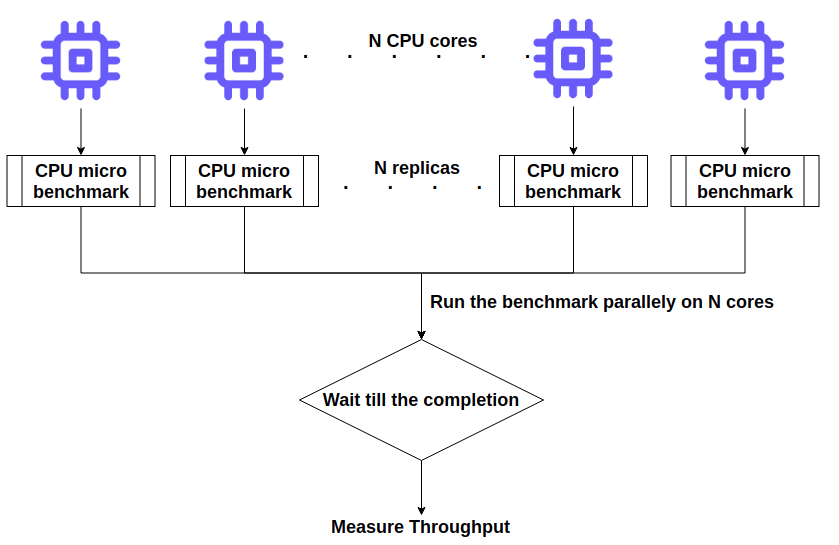
\includegraphics[width=\linewidth]{Pictures/cpu_micro_benchmark.png}
  \caption{CPU micro benchmark experiment setup}
  \label{cpu_micro_bench_mark}
  \Description{CPU micro benchmark experiment setup}
\end{figure}

As shown in the figure \ref{cpu_micro_bench_mark}, we have pinned each replica of CPU micro benchmark to a CPU core using Linux taskset command. By altering the value of $N$, the number of CPU cores available, between 1 to 64, we have run $N$ replicas parallely on $N$ CPU cores and measured the throughput, since all the $N$ CPU cores are completely utilized the throughput we measured is the maximum throughput $Throughput_{max}(N)$

The figure \ref{cpu_micro_bench_mark_throughput}, shows that, when the number of CPU cores $N$ increases, the observed throughput, $Throughput_{max}(N)$ increases. But when the number of CPU cores $N>32$, then the difference between the values of the observed  $Throughput_{max}(N)$  and the ideal $Throughput_{max}(N)$ is slightly high. To measure the scaling of throughput, we calculated the scalability factor with $N$ CPU cores, $S(N)$ using the equation \ref{eq:1}. The scalability factor we got for 64 CPU cores is 48, but the ideal  S(64) value is 64. By these results we came to the conclusion the even for a raw CPU micro benchmark 48 is the best scalability factor we can get with 64 CPU cores.


\begin{figure}[!htb]
  \centering
  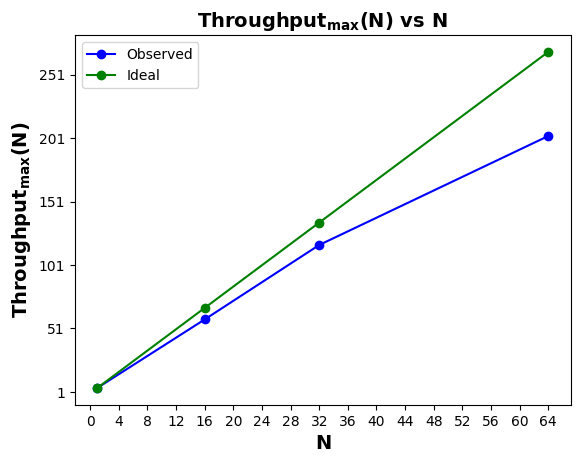
\includegraphics[width=\linewidth]{Pictures/cpu_micro_benchmark_throughput.png}
  \caption{CPU micro benchmark throughput plot}
  \label{cpu_micro_bench_mark_throughput}
  \Description{CPU micro benchmark throughput plot}
\end{figure}
\subsection{Evalpro micro benchmark}\label{evalpro_micro_benchmark_section}
To find the reason for scalability limitation shown in the section \ref{baseline_64} of Evalpro application, we designed a Evalpro micro benchmark because the micro benchmark has few lines of code, it will be easier to perform low level bottleneck analysis on it  compared to the entire application. The  Evalpro micro benchmark runs the auto-grading session i.e compilation of the code, execution of the object code generated by compilation and comparing the expected output with  the actual output. For compilation we used g++ compiler. The auto-grading session is run in a tight loop of 75 iterations. The Evalpro micro benchmark is run on the server having 64 CPU cores shown in the table \ref{tab:hardware_64_cores}.
\begin{figure}[!htb]
  \centering
  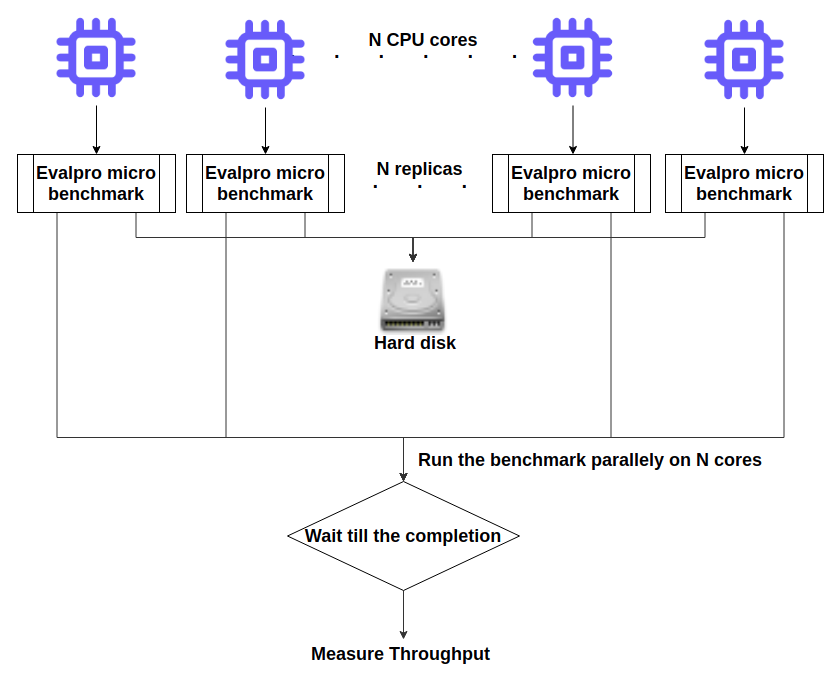
\includegraphics[width=\linewidth]{Pictures/evalpro_micro_benchmark.png}
  \caption{Evalpro micro benchmark experiment setup}
  \label{evalpro_micro_bench_mark}
  \Description{Evalpro micro benchmark experiment setup}
\end{figure}

As shown in the figure \ref{cpu_micro_bench_mark}, we have pinned each replica of Evalpro micro benchmark to a CPU core using Linux taskset command and all the Evalpro micro benchmark replicas use the hard disk to read and write files while running the Evalpro auto-grader session. By altering the value of $N$, the number of CPU cores available, between 1 to 64, we have run $N$ replicas parallely on $N$ CPU cores and measured the throughput, since all the $N$ CPU cores are completely utilized the throughput we measured is the maximum throughput $Throughput_{max}(N)$

\begin{figure}[!htb]
  \centering
  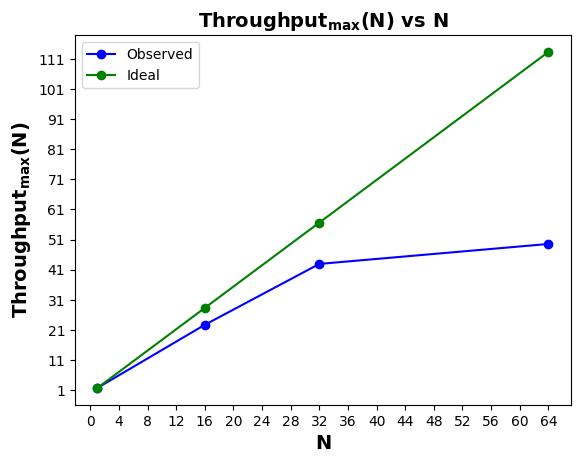
\includegraphics[width=\linewidth]{Pictures/evalpro_micro_benchmark_throughput.png}
  \caption{Evalpro micro benchmark throughput plot}
  \label{evalpro_micro_bench_mark_throughput}
  \Description{Evalpro micro benchmark throughput plot}
\end{figure}

The figure \ref{evalpro_micro_bench_mark_throughput}, shows that, when the number of CPU cores $N$ increases, the observed throughput, $Throughput_{max}(N)$ increases. But when the number of CPU cores $N>32$, then the difference between the values of the observed  $Throughput_{max}(N)$  and the ideal $Throughput_{max}(N)$ is much higher than the difference observed for the CPU micro benchmark shown in the figure \ref{cpu_micro_bench_mark_throughput}. To measure the scaling of throughput, we calculated the scalability factor with $N$ CPU cores, $S(N)$ using the equation \ref{eq:1}. The scalability factor we got for 64 CPU cores is 28, but the ideal  S(64) value is 64.

\begin{figure}[!htb]
  \centering
  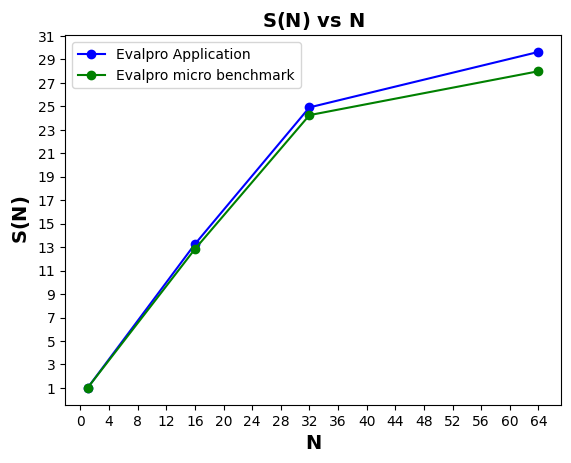
\includegraphics[width=\linewidth]{Pictures/scalability_comparision.png}
  \caption{ Evalpro Application and Evalpro micro benchmark comparison}
  \label{evalpro_scalability_comparision}
  \Description{Evalpro Application and Evalpro micro benchmark comparison}
\end{figure}


We have compared the Evalpro application's  baseline scalability factor calculated in section \ref{baseline_64} with the Evalpro micro benchmark's scalability factor calculated above. As shown in the figure \ref{evalpro_scalability_comparision}, Evalpro application and micro benchmark scalability factor $S(N)$ values are very close. Since  the scalability factor of Evalpro application and Evalpro micro benchmark are almost same, therefore we hypothesise that the reason for scalability limitation of Evalpro application will be same as the reason for Evalpro micro benchmark. Therefore we have performed bottleneck analysis on the Evalpro micro benchmark to find the reason for its scalability limitation. The next section briefly describes about bottleneck analysis on the Evalpro micro benchmark.

\section{Micro benchmark Bottleneck Analysis}\label{micro_benchmark_bottleneck_analysis}

For Evalpro micro benchmark, we observed  limitation in the scalability factor $S(N)$ for $N>32$ in the previous section. We performed the low level bottleneck analysis on the Evalpro micro benchmark to find the reason for its scalability limitation. Moreover since the micro benchmark has few lines of code, it will be easier to perform low level bottleneck analysis on the micro benchmark compared to the entire application. In this section we have performed low level bottleneck analysis on the Evalpro micro benchmark.

\subsection{Using Tmpfs in place of Hard Disk}
Tmpfs is a in-memory file system which stores file in the memory instead of disk. We hypothesised that the usage of disk by multiple Evalpro micro benchmark replicas, as shown in the figure \ref{evalpro_micro_bench_mark}, is limiting its scalability factor $S(N)$ for $N>32$. So, as shown in the figure \ref{evalpro_micro_benchmark_tmpfs}, we used Tmpfs instead of hard disk to store,read files while running Evalpro auto-grading session
\begin{figure}[!htb]
  \centering
  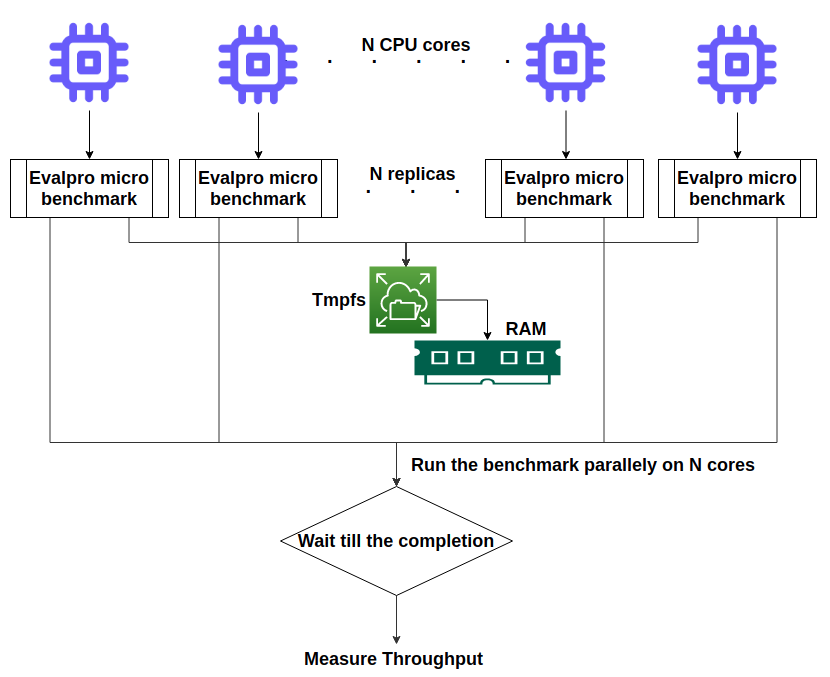
\includegraphics[width=\linewidth]{Pictures/evalpro_micro_benchmatk_tmpfs.png}
  \caption{ Evalpro micro benchmark using Tmpfs}
  \label{evalpro_micro_benchmark_tmpfs}
  \Description{Evalpro micro benchmark using Tmpfs}
\end{figure}


The throughput we measured using Tmpfs with $N$ CPU cores, $Throughput_{max}(N)$ is compared with $Throughput_{max}(N)$ using Hard disk. From the figure \ref{evalpro_micro_benchmark_tmpfs_comparision}, it is clear that using Tmpfs in place of hard disk to store,read files  makes no significant difference in the throughput. Thus we came to the conclusion that using disk to store,read files while running Evalpro auto-grader session is not the bottleneck i.e not the reason for limitation in the scalability.

\begin{figure}[!htb]
  \centering
  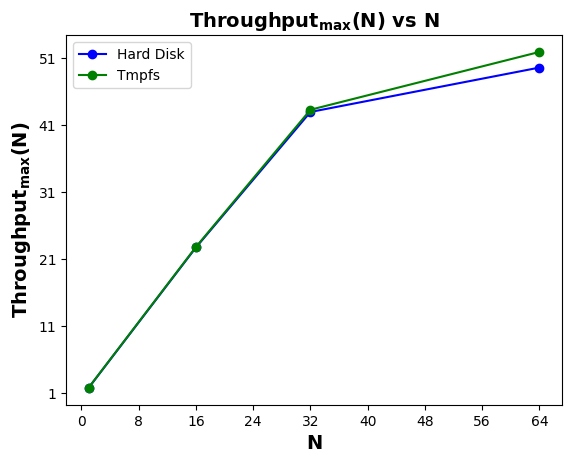
\includegraphics[width=\linewidth]{Pictures/hard_disk_tmpfs_comparision.png}
  \caption{ Comparison of Tmpfs and Hard disk}
  \label{evalpro_micro_benchmark_tmpfs_comparision}
  \Description{Comparison of Tmpfs and Hard disk}
\end{figure}

\subsection{Low level bottleneck analysis using PERF}

PERF tool[cite] is used to closely monitor a workload to get information about different types of software, hardware events raised during the execution of the workload. We used  PERF tool to count the occurrence of the following events during the execution of the Evalpro micro benchmark.
\begin{itemize}
\item {\texttt{LLC-loads}}: counts the number of memory accesses which load data from the  Last level cache  i.e L3 cache.
 \item {\texttt{LLC-load-misses}}: counts the number of memory accesses which resulted in cache miss while trying load  the data from Last level cache  i.e L3 cache.
\item {\texttt{LLC-stores}}:  counts the number of memory accesses which store data into the  Last level cache  i.e L3 cache 
\item {\texttt{LLC-store-misses}}: counts the number of memory accesses which resulted in cache miss while trying to store  the data into the Last level cache  i.e L3 cache.
\item {\texttt{page-faults}}: counts the number of memory accesses which resulted in page faults.
\item {\texttt{instructions}}: counts the number of instructions present in the workload.
\item {\texttt{branches}}: counts the number of instructions which resulted in taking the branch.
\item {\texttt{branch-misses}}: counts the number of branch instructions which the branch predictor wrongly predicted as not a branch instruction.
\end{itemize}

\begin{figure}[!htb]
  \centering
  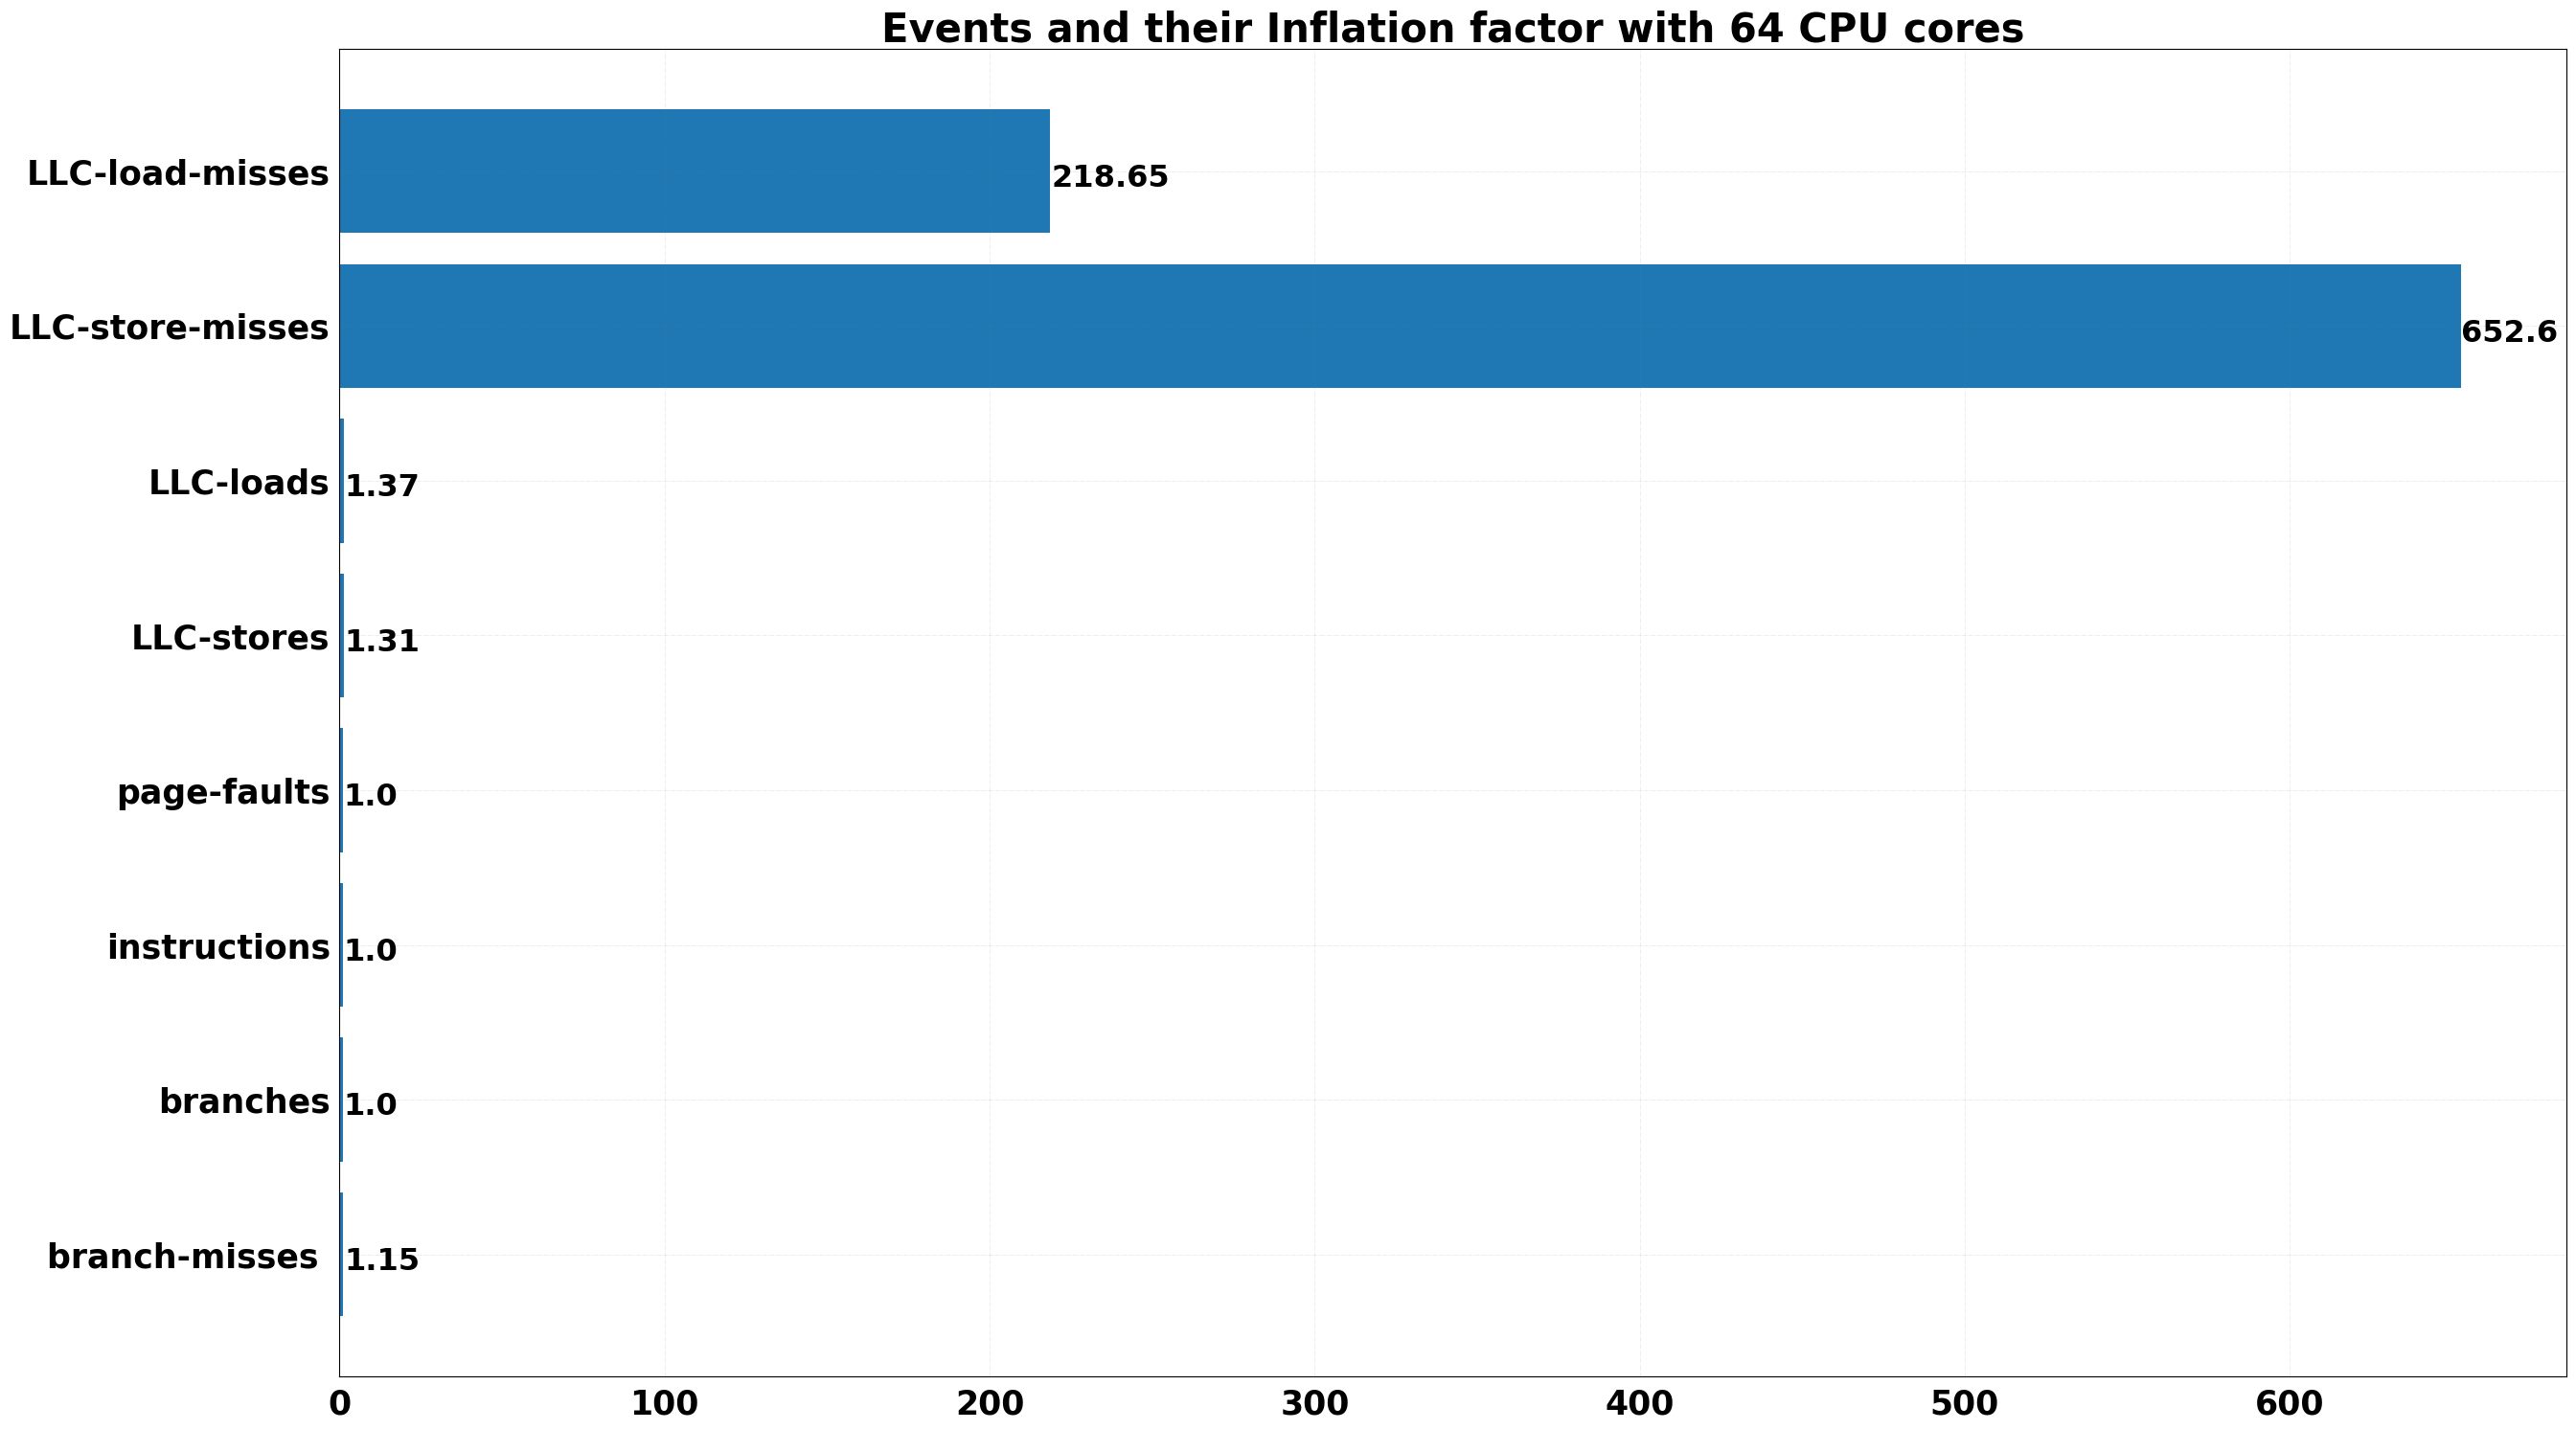
\includegraphics[width=\linewidth]{Pictures/perf_tool_results.png}
  \caption{Inflation factor of Events by Perf tool}
  \label{perf_results}
  \Description{Comparison of Tmpfs and Hard disk}
\end{figure}


 Using the PERF tool, we have measured the occurrence count of the events by running Evalpro micro benchmark with the experiment setup shown in the figure \ref{evalpro_micro_bench_mark}. We altered the number of CPU cores and number of Evalpro micro benchmark replicas, $N$ from 1 to 64. To measure the inflation in the occurrence of an event when increasing the number of CPU cores $N$, we define the Inflation factor. As shown in the equation \ref{eq:2}, for an event the Inflation factor with $N$ CPU cores is  $Inflation\_factor_{event}(N)$, which is equal to the ratio of occurrence count of the event with $N$ CPU cores normalized to a single CPU core, $Normalized\_count_{event}(N)$ and the occurrence count of the event  with a single CPU core, $Count_{event}(1)$.

\begin{equation}
  Inflation\_factor_{event}(N)=\frac{Normalized\_count_{event}(N)}{Count_{event}(1)}
  \label{eq:2}
\end{equation}

As shown in the figure \ref{perf_results}, the value of the  Inflation factor with 64 CPU cores, $Inflation\_factor_{event}(64)$ is very high for LLC-load-misses and LLC-store-misses. But  for other  events the value of $Inflation\_factor_{event}(64)$ is almost 1, which is negligible. By these results it is clear that LLC-load-misses and LLC-store-misses have been disproportionately inflated when the number of CPU cores $N>32$.

To find the  program in the Evalpro micro benchmark which is causing the  disproportionate inflation of LLC load and store misses, we have used PERF tool to find percentage of LLC misses at program level. As shown the figure \ref{llc_misses_gplusplus}, it is clear that  compared to 1 CPU core, on 64 CPU cores, the percentage of LLC misses i.e LLC-load-misses and LLC-store-misses by g++ program is very high. 

\begin{figure}[!htb]
  \centering
  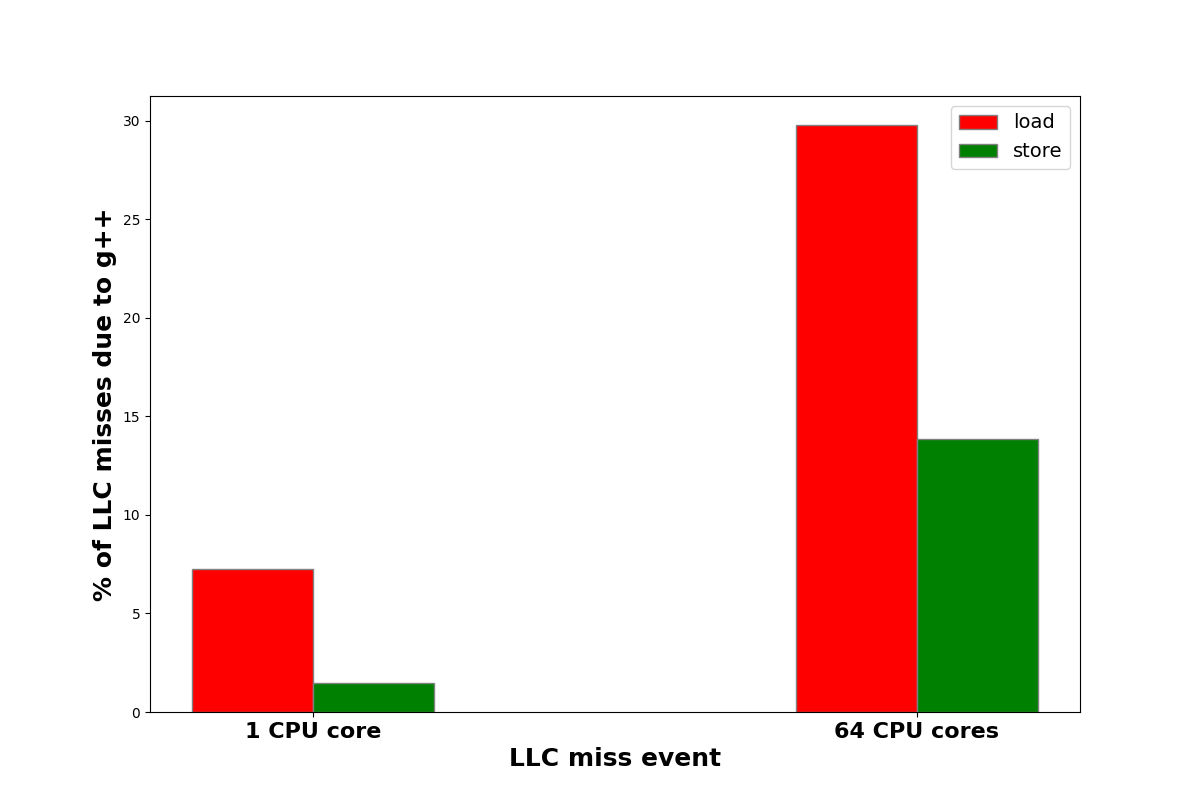
\includegraphics[width=\linewidth]{Pictures/llc_misses_g++.png}
  \caption{Increase in LLC misses with CPU cores by g++ }
  \label{llc_misses_gplusplus}
  \Description{Increase in LLC misses  with CPU cores by g++}
\end{figure}


From the above results it is clear that even though the L3 CPU cache size is 80MB,  when the L3 cache is shared with 64 Evalpro micro benchmark replicas each running on a separate CPU core then due to the memory intensive nature of g++ program, the L3 CPU cache is becoming the bottleneck. Thus the limitation in CPU cache size is the reason for scalability limitation of Evalpro micro benchmark. 


\section{PERF analysis on }

To validate our hypothesis at the end of the section \ref{evalpro_micro_benchmark_section},  that the reason for scalability limitation of Evalpro micro benchmark  i.e  CPU cache is also the reason for scalability limitation of Evalpro application, we have compared the maximum throughput we observed with 16 CPU cores in our initial baseline experiments, shown in the section \ref{baseline_16} with the  maximum throughput we observed with 16 CPU cores, in our final baseline experiments, shown in the section \ref{baseline_64}. The server used for initial baseline experiments is a 16 CPU core single socket server with 20MB CPU cache (L2+L3), where as the server used for final baseline experiments is a 64 CPU core two socket server with 88MB CPU cache (L2+L3)  i.e each socket has 32 CPU cores, 40MB L3 CPU cache and 8MB L2 CPU cache. The CPU's corresponding to the two servers used for initial and final baseline experiments belong to the same Intel(R) Xeon(R) Processor E5 v4 family.

As shown in the figure \ref{throughput_cache_graph}, in our initial baseline experiments  when 16 CPU cores are using 20MB CPU cache, then the observed  throughput, $Throughput_{max}(16)$ was 3.4 requests per second. Using the CPU of the same family, in our final  baseline experiments, for 16 CPU cores when the CPU cache size is increased to more than twice i.e 48MB, then the observed  throughput, $Throughput_{max}(16)$ was 8.75 requests per second i.e throughput was increased to more than twice. From these results it is clear that when the CPU cache size is increased then the throughput increased proportionally to the CPU cache size. Therefore our hypothesis that the  CPU cache is the bottleneck for the Evalpro application turns out to be true.

For our Evalpro application, linear scaling of throughput can be achieved by increasing the number of CPU cores only up to certain number of CPU cores After that since the L3 CPU cache is shared among the CPU cores,  due to memory intensive nature of compilation the throughput didn't scale linearly by increasing the number of CPU cores. Hence to get the linear scaling of the throughput, CPU cache size also should be incremented with the CPU cores. The next section concludes this paper.

\begin{figure}[!htb]
  \centering
  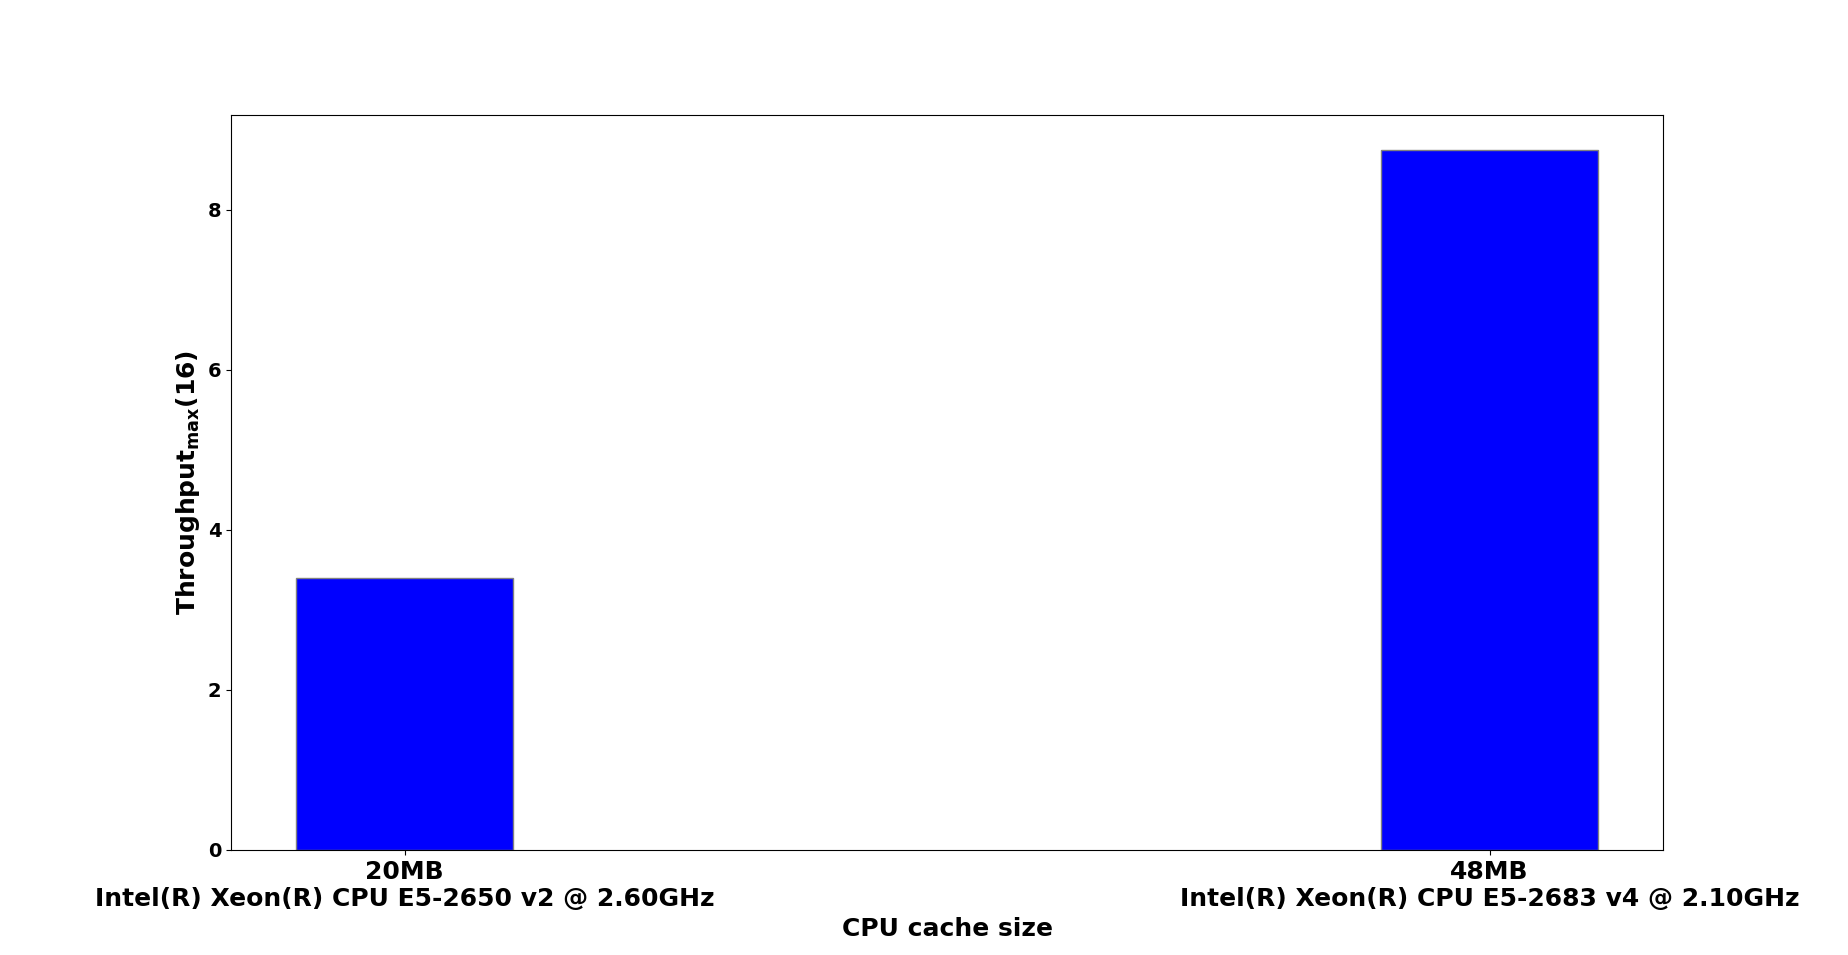
\includegraphics[width=\linewidth]{Pictures/cpu_cache_throughput.png}
  \caption{Throughput vs CPU cache size }
  \label{throughput_cache_graph}
  \Description{Increase in throughput  with CPU cache size}
\end{figure}


\section{Conclusion}\label{conclusion}
We have started with the baseline experiments and found that the throughput scaling of our Evalpro application is not proportional with the increase in the CPU cores. Therefore we tried to find the bottlenecks, which limit the scalability and found that there are no application bottlenecks. After that we tried horizontal scaling for better isolation, in which we tried Container based virtualization using docker swarm, Hardware assisted virtualization using KVM and used MongoDB in place of disk to store the files but got no improvement in the scalability. We developed two micro benchmarks i.e CPU micro benchmark and Evalpro micro benchmark to find the best scalability that can achieved for a raw CPU workload and the Evalpro application respectively. We performed low level bottleneck analysis on the Evalpro micro benchmark to  reason for its scalability limitation, in which we used PERF tool and found that L3 CPU cache misses have been disproportionately inflated due to g++ compilation from which we hypothesised that  CPU cache size is the bottleneck for Evalpro application. We also found that increasing  CPU cache size increases the throughput of the Evalpro application proportionally, which validates our hypothesis that CPU cache is the bottleneck. Therefore we conclude that linear scaling of throughput can be achieved by increasing the number of CPU cores only up to certain number of CPU cores, after that to get the linear scaling of the throughput, cache size also should be incremented with the CPU cores.

\section{Summary}
\begin{figure*}
  \centering
  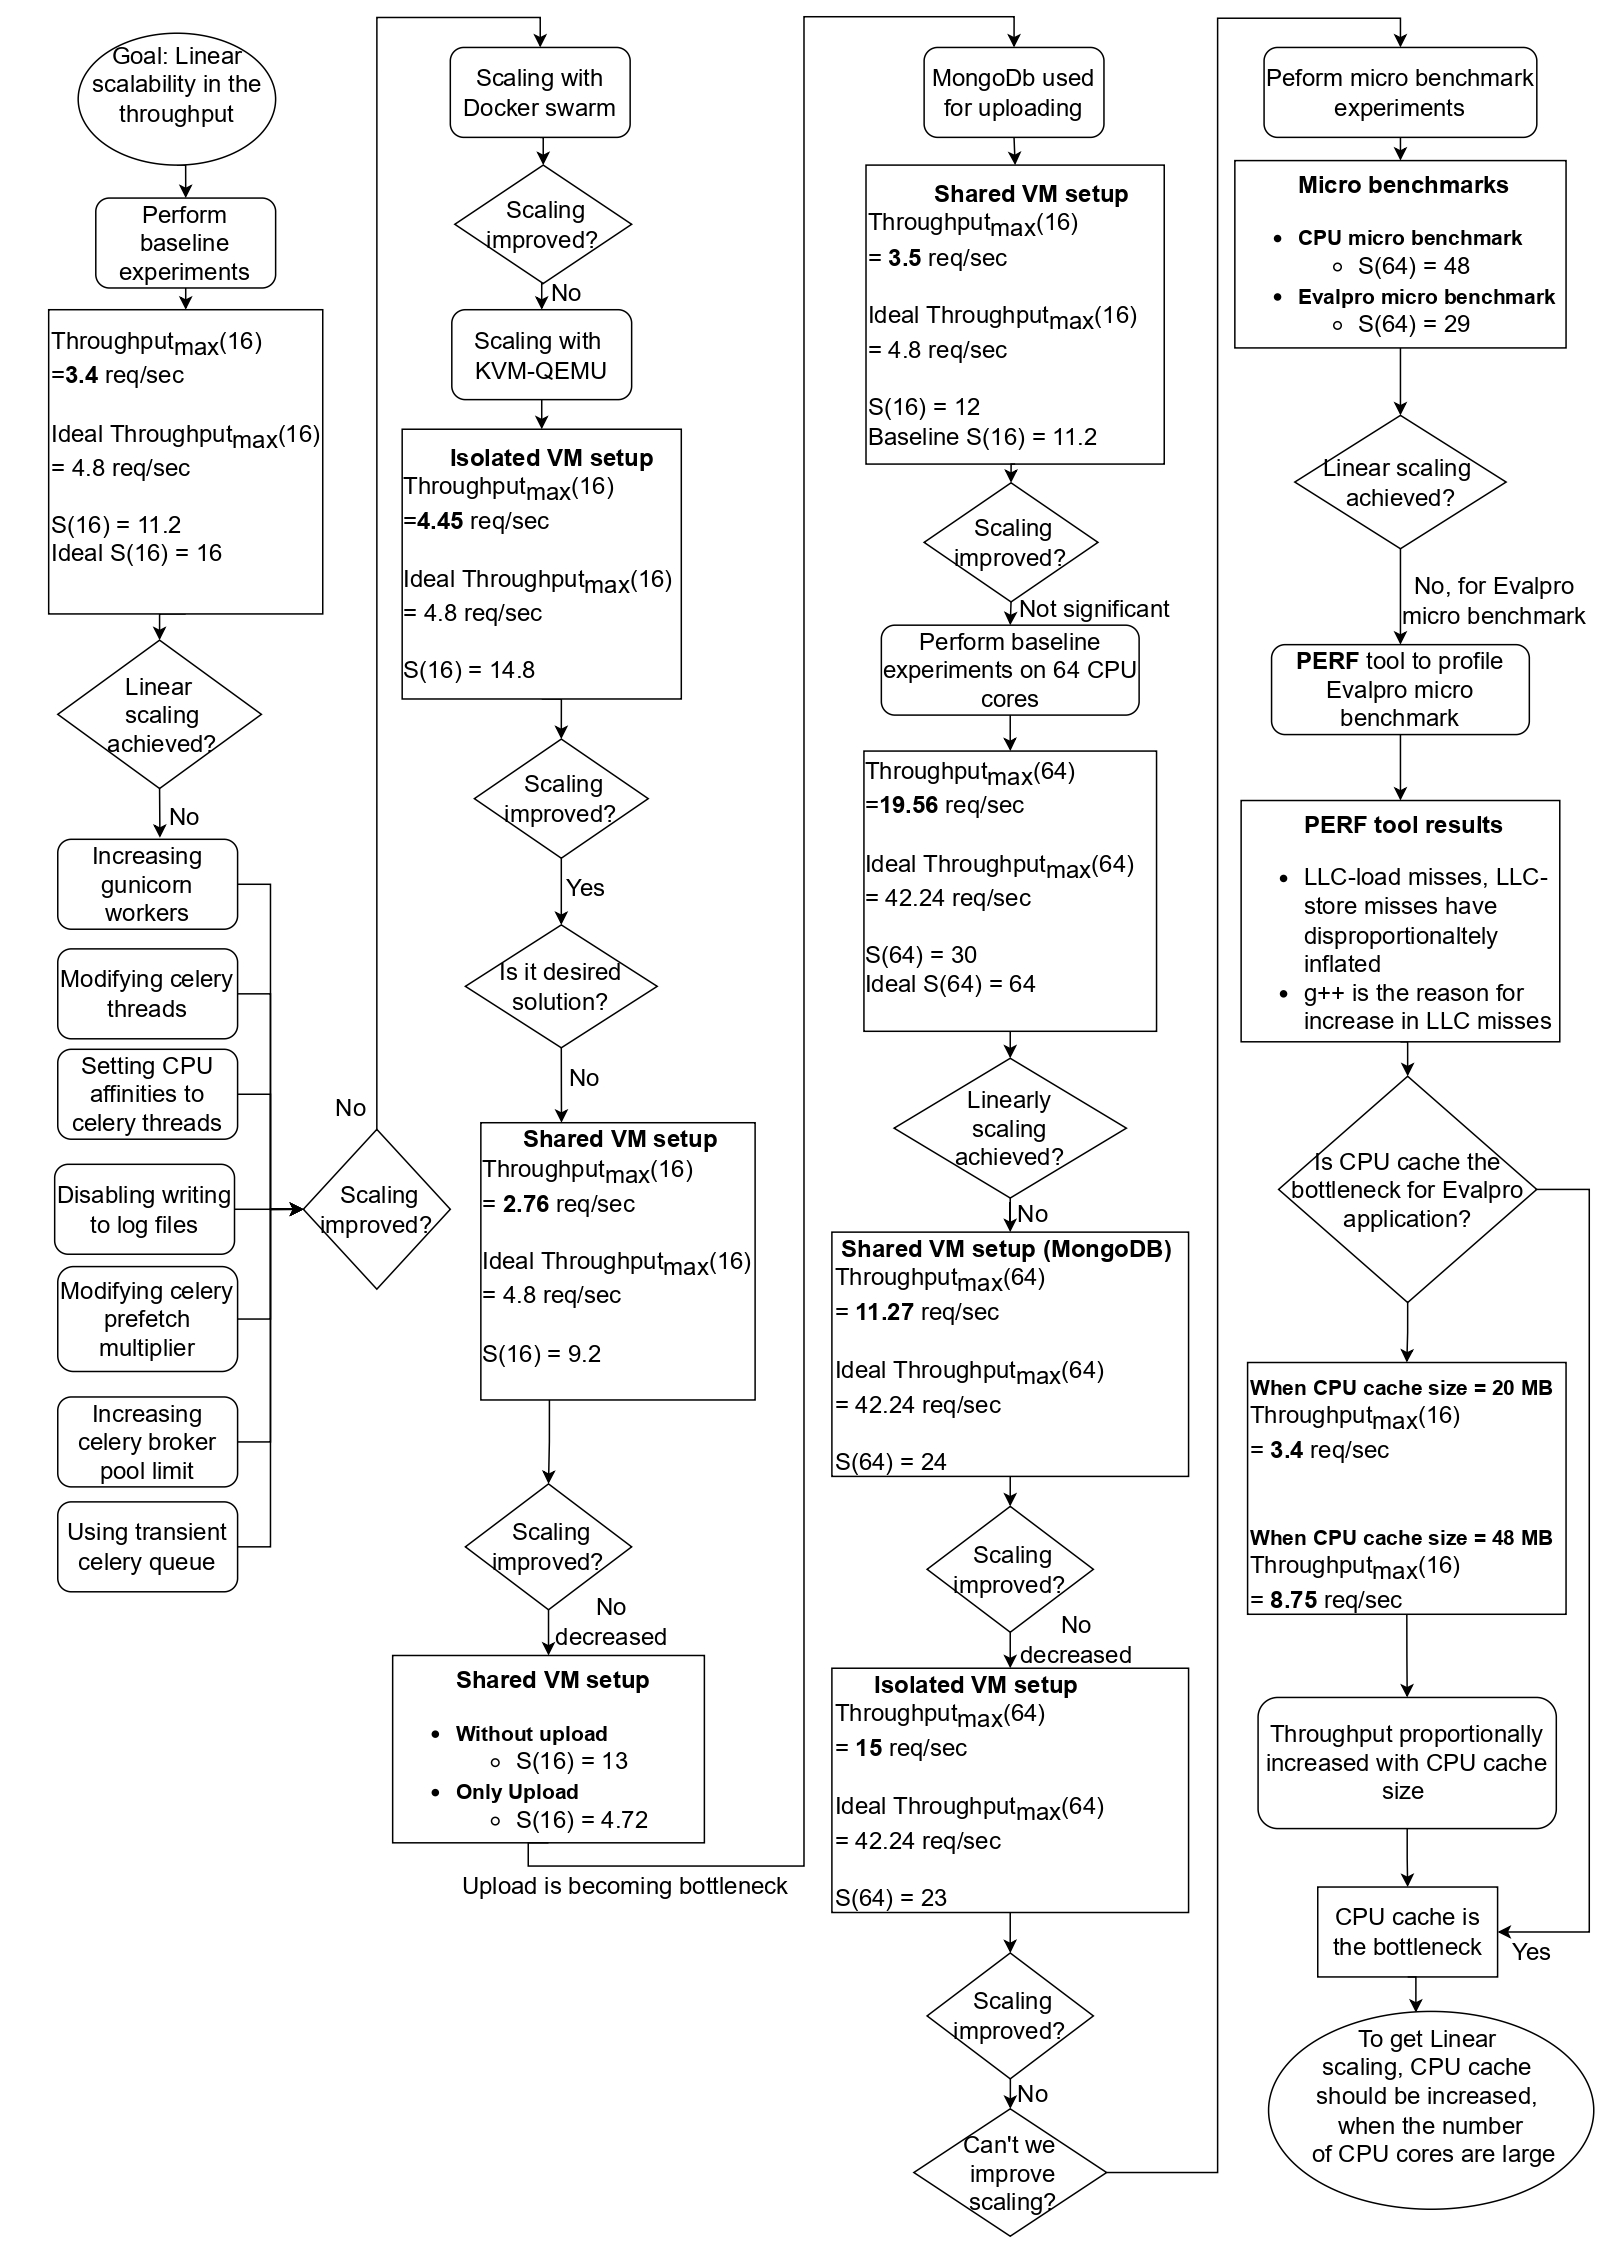
\includegraphics[scale=0.6]{Pictures/paper_summary.jpg}
  \caption{Summary}
  \label{paper_summary}
  \Description{Overall summary of work}
\end{figure*}




\begin{acks}

\end{acks}

\bibliographystyle{ACM-Reference-Format}
\bibliography{scalability-paper}

\end{document}
\endinput
%%
%% End of file `sample-sigconf.tex'.
